

\def \currentAuthor {Lukas Vogel} %so kann jederzeit der Autor geändert werden -> wird in der Fusszeile angezeigt.


\chapter{Einleitung}
Diese Diplomarbeit befasst sich mit der Entwicklung des Prototyps: NeXt. Das Produkt ist eine spielbare Version eines Computerspiels in dem sogenannte Jump and Run-Elemente, Puzzele-Elemente sowie Zeitmanagement-Elemente beinhaltet sind. Das Projekt wurde in Verbindung mit der Firma ClockStone Softwareentwicklung GmbH. erarbeitet. Interesse könnte diese Dokumentation bei jedem erwecken, der sich über Spielentwicklung in Verbindung mit der Unity-Engine informieren will. Des Weiteren werden auch die Aspekte des Projektmanagements dieser Arbeit dargelegt.

\chapter{Projektmanagement}

\section{Metainformationen}
\subsection{Team}

	\begin{figure}[H]
	\centering
		
\includegraphics[width=4cm]{images/LukasVogel.png}
		\caption{Lukas Vogel}		
	\end{figure}

	\textbf{Name:} Lukas Vogel\\
\textbf{Funktion:} Projekt Leiter\\
\textbf{Wohnort:} Hohenems\\
\textbf{E-Mail:} lvogel@tsn.at\\
\textbf{Aufgabenbereiche:} \begin{itemize}
	\item GUI
	\item Leveldesign
	\item Dokumentation
\end{itemize}
\begin{figure}[H]
	\centering
	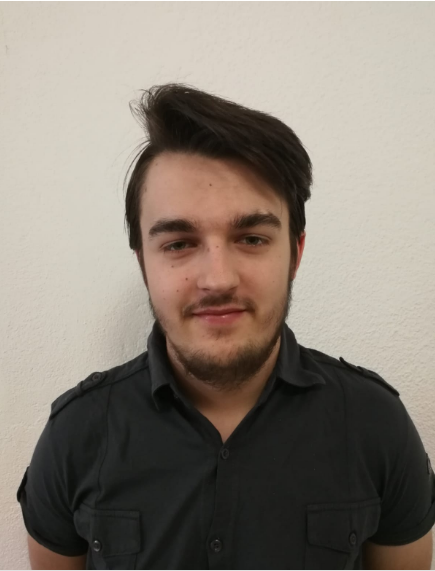
\includegraphics[width=4cm]{images/Michael.PNG}
	\caption{Michael Leitner}
\end{figure}
	\textbf{Name:} Micahel Leitner\\
\textbf{Funktion:} Team Mitglied\\
\textbf{Wohnort:} Oberperfuss\\
\textbf{E-Mail:} mleitner@tsn.at\\
\textbf{Aufgabenbereiche:} \begin{itemize}
	\item Steuerung
	\item Tiem-Rift-Prinzip
	\item Dokumentation
\end{itemize}
\newpage
\subsection{Betreuer}
Seitens der Schule hat sich Herr Claudio Landerer bereiterklärt unser Projekt zu betreuen. Er brachte uns in seinem Unterricht das Programmieren bei.
	\begin{figure}[H]
		\centering
		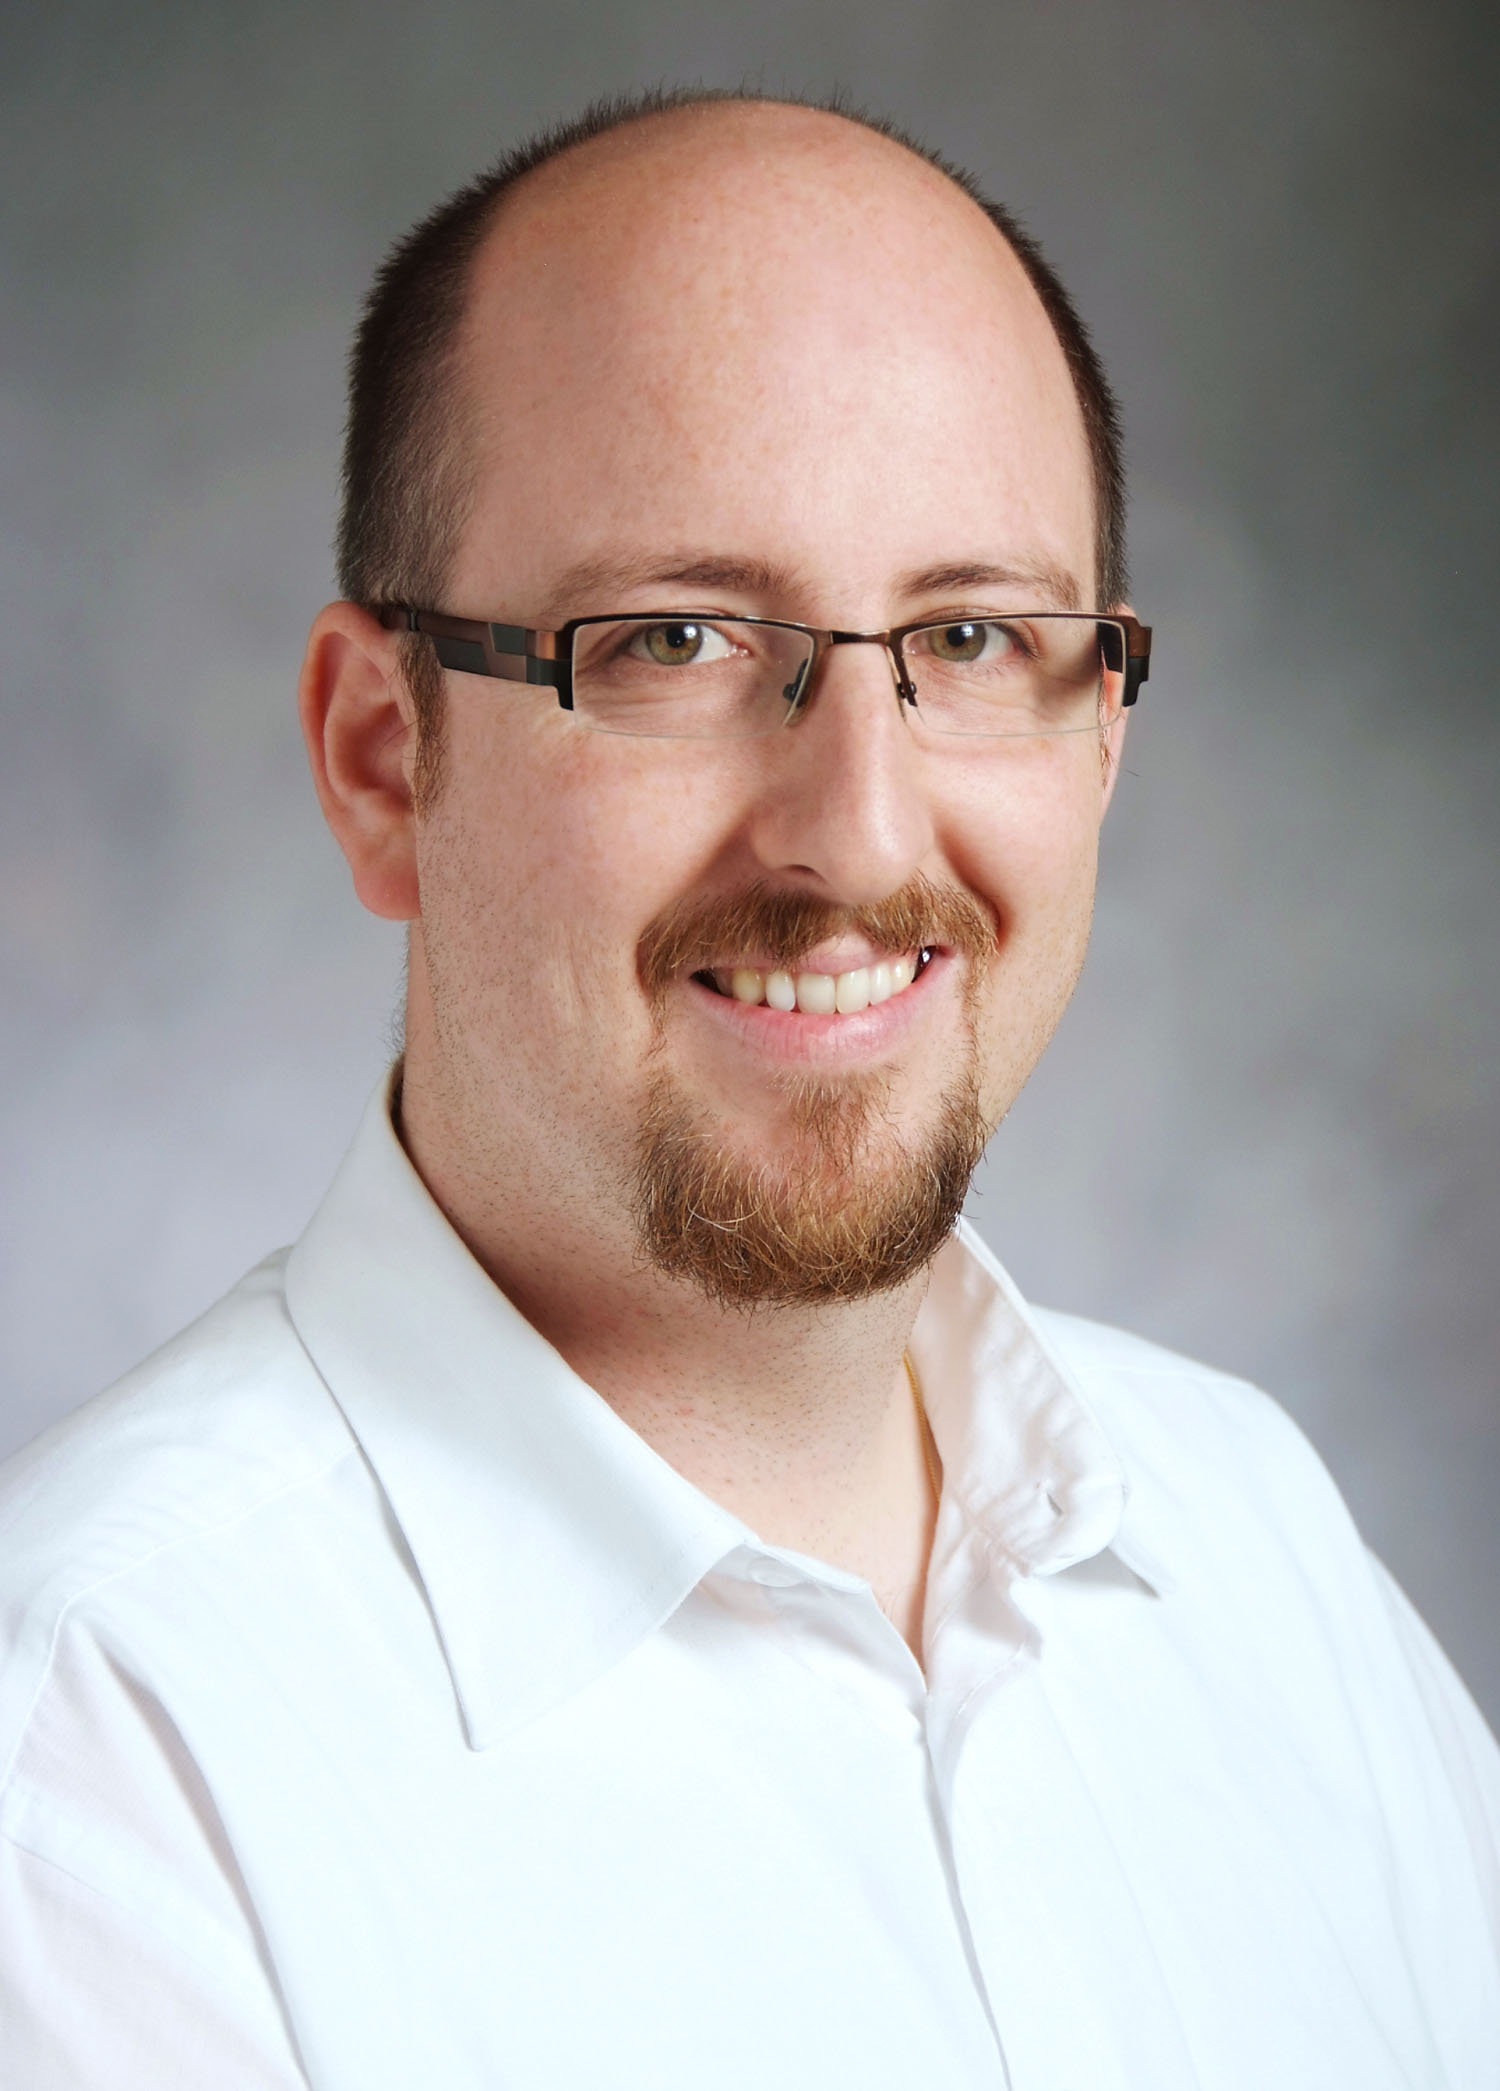
\includegraphics[width=4cm]{images/Landerer_Claudio.jpg}
		\caption{Mag. Claudio Landerer}
	\end{figure}
		
\newpage
\subsection{Partner}
\begin{figure}[H]
	\centering
	
\includegraphics[]{images/ClockstoneLogo.png}
	\caption{ClockStone Softwareentwicklung GmbH}
\end{figure}
Unser Partner während der Diplomarbeit war die Firma ClockStone Softwareentwicklung GmbH. ClockStone ist ein Spielentwicklungsunternehmen mit Sitz in Innsbruck, das im Jahr 2006 gegründet wurde. Einige ihrer Produkte, wie zum Beispiel Bridge Constructor, sind weltweit bekannt und sehr beliebt. 


\subsection{Ansprechpartner}
Unser Ansprechpartner des Unternehmens war Michael Schiestl. Er unterstütze uns bei Fragen bezüglich der Spielentwicklung und es war äußerst angenehm mit ihm zu arbeiten.

\begin{figure}[H]
	\centering
	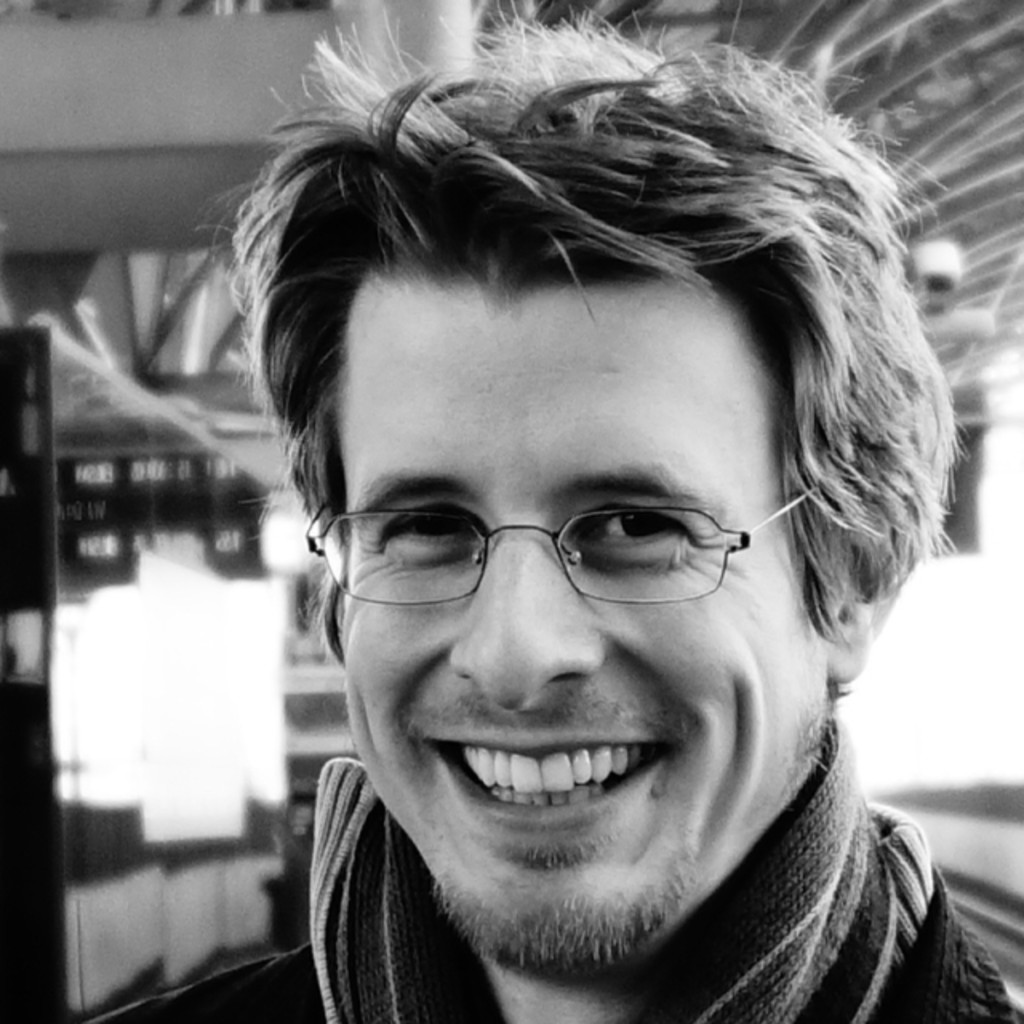
\includegraphics[width=4cm, height=4cm]{images/michaelschiestl.jpg}
	\caption{Michael Schiestl}
\end{figure}
\section{Vorerhebungen}
\subsection{Projektzieleplan}
\def \currentAuthor {Michael Leitner} Das Ziel unseres Projekts ist es ein spielbares, unterhaltendes und einfach bedienbares Computer Spiel zu entwickeln. Die Meilensteine sollen termingerecht realisiert werden und es soll pünktlich bis zur Projektabgabe im Juni fertig gestellt werden.
\newpage
\subsection{Projektumfeld}
\def \currentAuthor {Lukas Vogel} %so kann jederzeit der Autor geändert werden -> wird in der Fusszeile angezeigt.
\subsubsection{Stakeholder-Analyse}
Die Ergebnisse der Stakholder-Analyse zu sehen in Tabelle \ref{Stakeholder-Analyse}:
\begin{table}[H]
		
	\renewcommand{\arraystretch}{1.5}
		\begin{tabular}{|p{3cm}|p{6cm}|p{3cm}|p{1.5cm}|p{1.5cm}|}
			\hline
			\textbf{Stakeholder} & \textbf{Beschreibung} & \textbf{Einstellung} & \textbf{Nähe zum Projekt} & \textbf{Einfluss} \\
			\hline
			Projektteam & Das Team ist dem Projekt positiv eingestellt und hofft, sich neues Wissen aneignen zu können. & sehr positiv & 10 & 10\\
			\hline
			Landerer Claudio & Betreuer des Projekts. & neutral & 9 &10\\
			\hline
			ClockStone Softwareentwicklung GmbH.& Projektpartner der Diplomarbeit & positiv & 9 & 10\\
			\hline
			Stefan Walch & Direktor der Schule und Studienkoordinator & neutral& 5 & 10\\
			\hline
			Andere Lehrpersonen & Die anderen Lehrpersonen des IT-Kollegs sind während allen Präsentationen anwesend und können die Notengebung beeinflussen & neutral& 2 & 4\\
			\hline
			Mitschüler & Manche Klassenmitglieder spielen gerne am Computer in der Freizeit	& neutral bis positiv & 1 & 1\\
			\hline
		\end{tabular}
\caption{Stakeholder-Analyse}
\label{Stakeholder-Analyse}
	\end{table}
Die Einschätzung der Einstellung, der verschiedenen Stakeholder zum Projekt in Tabelle \ref{Stakeholder-Analyse} geht von sehr negativ über neutral bis zu sehr positiv. Der Einfluss auf die Diplomarbeit wiederum wird mit einer Skala von 1-10 beschrieben, wobei 1 keinen bzw. sehr wenig Einfluss repräsentiert und 10 eine sehr starken. Auch die Nähe zum Projekt wird von 1-10 skaliert, 1 repräsentiert weit entfernt vom Projekt und 10 sehr nah.

\subsubsection{Stakeholder-Diagramm}
\begin{figure}[H]
	\centering
	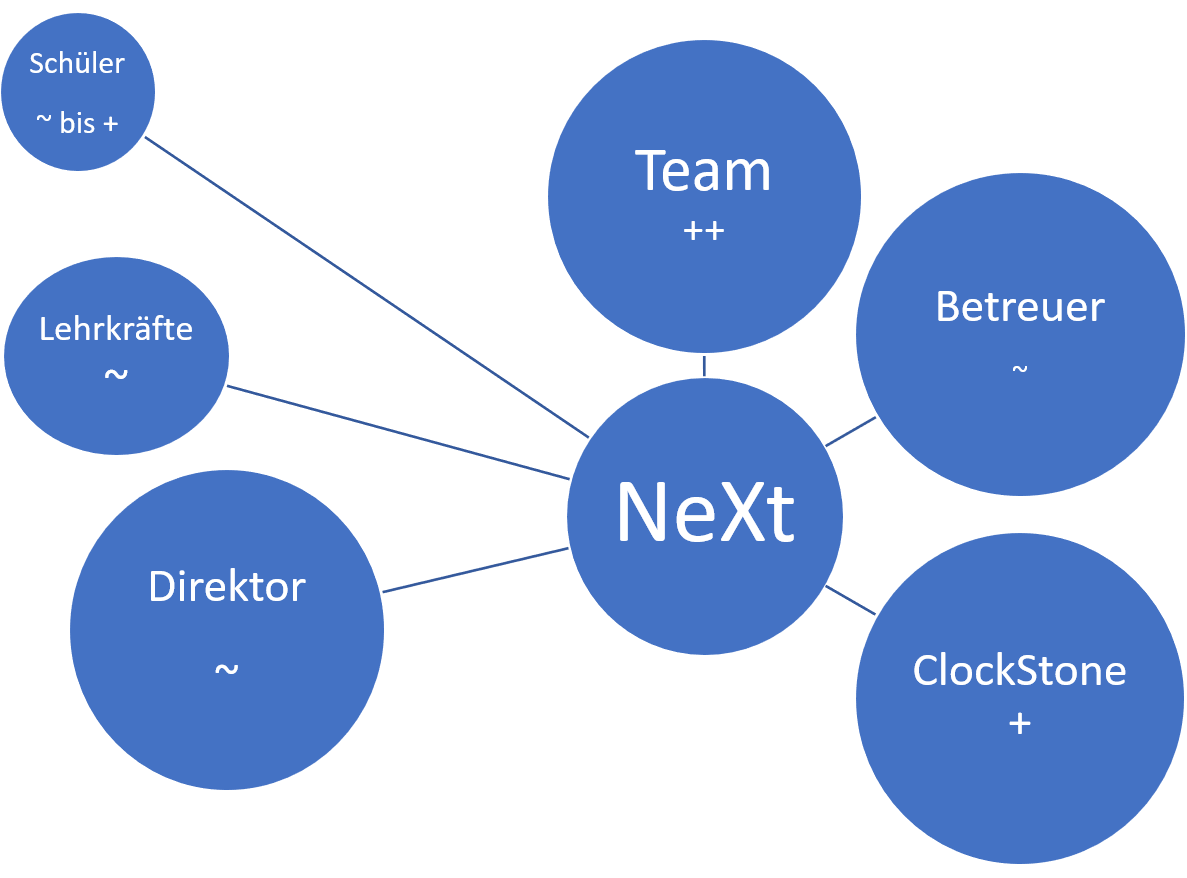
\includegraphics[width=16cm,height=8cm]{images/Projektumfeldanalyse.png}
	\captionbelow{Stakeholder-Diagramm}
	\label{Stakeholder-Diagramm}
\end{figure}
In diesem Diagramm, Abbildung \ref{Stakeholder-Diagramm} ist das Ergebnis der Tabelle \ref{Stakeholder-Analyse} graphisch dargestellt. Die Größe der Kreise zeigt den Einfluss, die Länge der Linien zwischen Stakeholder und NeXt die Nähe und die Zeichen (++ –> sehr positiv, –> neutral, – –> sehr negativ) unter dem Namen des Stakeholders dessen Nähe zum Projekt.

\subsection{Risikoanalyse}
\begin{figure}[H]
	\centering
	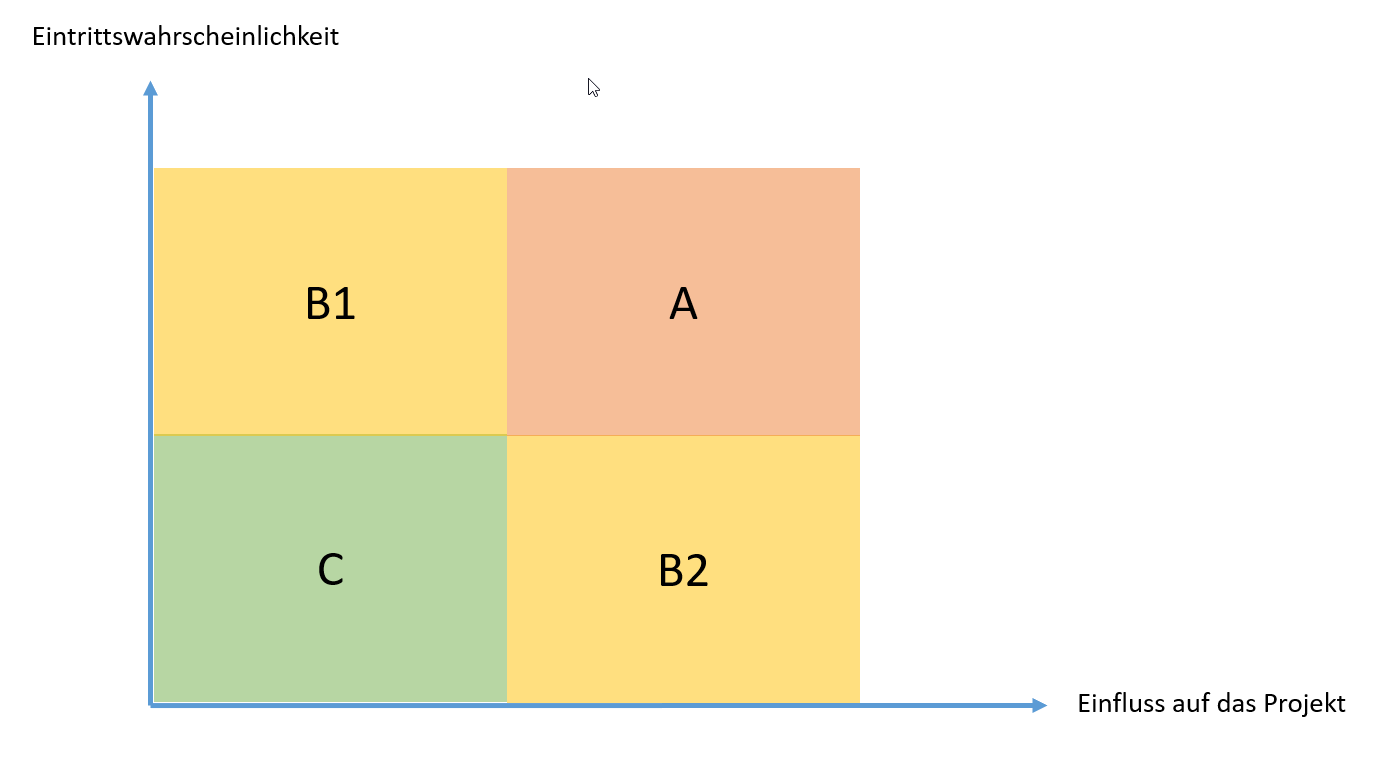
\includegraphics[width=16cm,height=8cm]{images/Risiko-Matrix.png}
	\caption{Matrix zur qualitativen Einordnung von Risiken}
	\label{MatrixRisiken}
\end{figure}
Die Matrix (\ref{MatrixRisiken}) wurde in vier Kategorien eingeteilt. Die Risiken werden dann zur jeweils passende Kategorie zugeordnet um diese dann besser einschätzen zu können. \cite[S. 141 -142]
Folgende Risiken sind aus der Projektumfeld-Analyse hervorgegangen und werden in Tabelle \ref{Risiko} beschrieben, bewertet und Maßnahmen gesetzt.


	\begin{table}[H]
			\centering
		\renewcommand{\arraystretch}{1.5}
		\begin{tabular}{|p{3cm}|p{5cm}|p{2cm}|p{5cm}|}
			\hline
			\textbf{Risiko} & \textbf{Beschreibung} & \textbf{Bewertung} & \textbf{Maßnahme} \\
			\hline
			Motivation des Teams & Die Motivation des Teams ist sehr wichtig. Wenn diese sinkt, verringert sich auch die Arbeitsmoral. Dies führt zu weniger Produktivität, was wiederum zum totalen Stillstand der Diplomarbeit führen kann. & A & Um die Wahrscheinlichkeit zu reduzieren sind am Anfang möglichst schnell Erfolgserlebnisse zu erzielen, dies steigert die Motivation sehr gut. Zusätzlich hilft es bei Problemen, nicht Stunden lang am Problem zu sitzen, sondern entweder an etwas Anderem zu arbeiten oder jemanden um Hilfe zu bitten.\\
			\hline
			Zufriedenheit des Betreuers & Herr Landerer ist der Betreuer des Projekts und wenn er nicht mit unseren Leistungen zufrieden ist kann er das Projekt stoppen. & B2 & \begin{itemize}
				\item laufende Berichterstattung
				\item laufender Fortschritt im Projekt
				\item bei Problemen oder Verzögerungen mit ihm reden
			\end{itemize}\\
		\hline
		Zufriedenheit des Partners & Die Firma ClockStone Softwareentwicklung GmbH soll wie der Betreuer mit dem Fortschritt und dem Projekt an sich zufrieden sein. Da auch sie im Extremfall das Projekt zum Stopp zwingen könne. & B2 & Auch hier kann eine laufende Berichterstattung und vor allem Meetings mit dem Partner helfen. Des Weiteren ist zu beachten, dass auch ihr Unternehmen Spiele entwickelt, dadurch können sie bei Problemen kontaktiert werden, was zu einer schnelleren Lösungsfindung führen kann und somit auch ihren Wünschen entspricht.\\
		 \hline
		\end{tabular}
	\end{table}
\newpage
\begin{table}[H]
	\centering	
		\renewcommand{\arraystretch}{1.5}
	\begin{tabular}{|p{3cm}|p{5cm}|p{2cm}|p{5cm}|}
		\hline
		Zufriedenheit des Direktors & Herr Walch ist auch für die Abnahme des Projekts zuständig. Wenn das Projekt seinen Anforderungen nicht entspricht, kann er das Projekt abbrechen. Darüber hinaus ist er bei den Präsentationen der Diplomarbeit anwesend, dort werden von den allen Lehrern auch Fragen zum Projekt gestellt. Wenn diese nicht eine fachlich kompetente Antwort bekommen, kann das einen negativen Einfluss auf das Projekt haben. & B2 & Um dieses Risiko abzuschwächen ist es besonders wichtig auf die Fragen und Anmerkungen von Herrn Walch einzugehen. Deswegen ist es essentiell sich gut auf die Präsentationen vor zu bereiten.\\
		\hline
		Zufriedenheit der anderen Lehrpersonen & Wie Herr Walch, sitzen auch andere Lehrpersonen während der Präsentation dabei und können Fragen zum
		Projekt stellen.
		 & C & Dieses Risiko kann mittels guter Vorbereitung bei den Präsentationen verringert werden. \\
		\hline
	\end{tabular}
		\caption{Risiko-Bewertung-Maßnahmen}
\label{Risiko}
\end{table}
\newpage
\section{Pflichtenheft}
\def \currentAuthor {Michael Leitner}
\subsection{Zielbestimmung}
Das Spiel „NeXt“ soll nach dem Time Rifts-Prinzip agieren. Das 2-dimensionale Spiel wird gemeistert durch:
\begin{itemize}
	\item koordinierte Zusammenarbeit aller Figuren
	\item Zeitmanagement
	\item Jump-and-Run Elemente
	\item Lösen von Puzzle-Elementen
\end{itemize}
\begin{figure}[H]
	\centering
	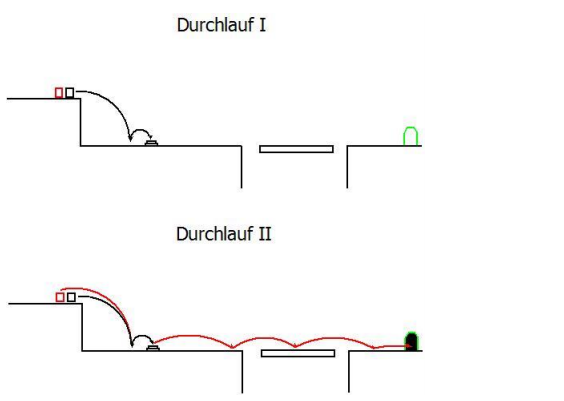
\includegraphics[width=10cm]{images/TimeRift.png}
\end{figure}
\textbf{Time Rift Prinzip}: Jeder Durchlauf hat ein Zeitlimit, dass Ziel sollte es sein durch die verschlossene Tür (grün) zu gehen.
\begin{itemize}
	\item Durchlauf I: Der/die Spieler/in bewegt Figur 1(schwarzes Rechteck) auf eine Bodenplatte. -> Tür öffnet sich. (bleibt offen solange die Bodenplatte betätigt ist)
	\item Durchlauf II: Figur 1 macht das selbe wieder (in Echtzeit) und der/die Spieler/in bewegt Figur 2 (rotes Rechteck) durch die Tür
\end{itemize}
Jedoch ist dieses Prinzip nicht nur auf 2 Durchgänge beschränkt.
\subsection{Produkteinsatz und Umgebung}
Die Zielgruppe dieses Spieles, ist jeder der sich einer Herausforderung stellen möchte. Durch das Time Rift-Prinzip wird eine große Herausforderung geboten. Spielbar wird dieses Spiel auf jedem Windows-Computer sein. Da auf gute Grafik verzichtet worden ist, muss der Computer auch nicht leistungsstark sein, um das Spiel ausführen zu können 
\subsection{Funktionalitäten}
\begin{itemize}
	\item MUSS-Anforderungen
	\begin{itemize}
		\item Funktional:
		\begin{itemize}
			\item Time Rift Prinzip-Implementiert
			\item Ein paar Level implementiert
		\end{itemize}
		\item Nicht-funktional
		\begin{itemize}
			\item Das Spiel soll einfach gesteuert werden
			\item Das Spiel soll Einschränkungen Spielbar sein.
		\end{itemize}
	\end{itemize}
	\item KANN-Anforderungen
	\begin{itemize}
		\item Funktional
		\begin{itemize}
			\item Ein Komplettes Level-Pack enthalten
			\item Erweiterte Steuerungsmöglichkeiten 
		\end{itemize}
		\item Nicht-funktional
		\begin{itemize}
			\item Das Spiel kann mit Musik unterlegt sein
		\end{itemize}
	\end{itemize}
\end{itemize}
\section{Planung}
\subsection{Projektstrukturplan}
\begin{figure}[H]
	\centering
	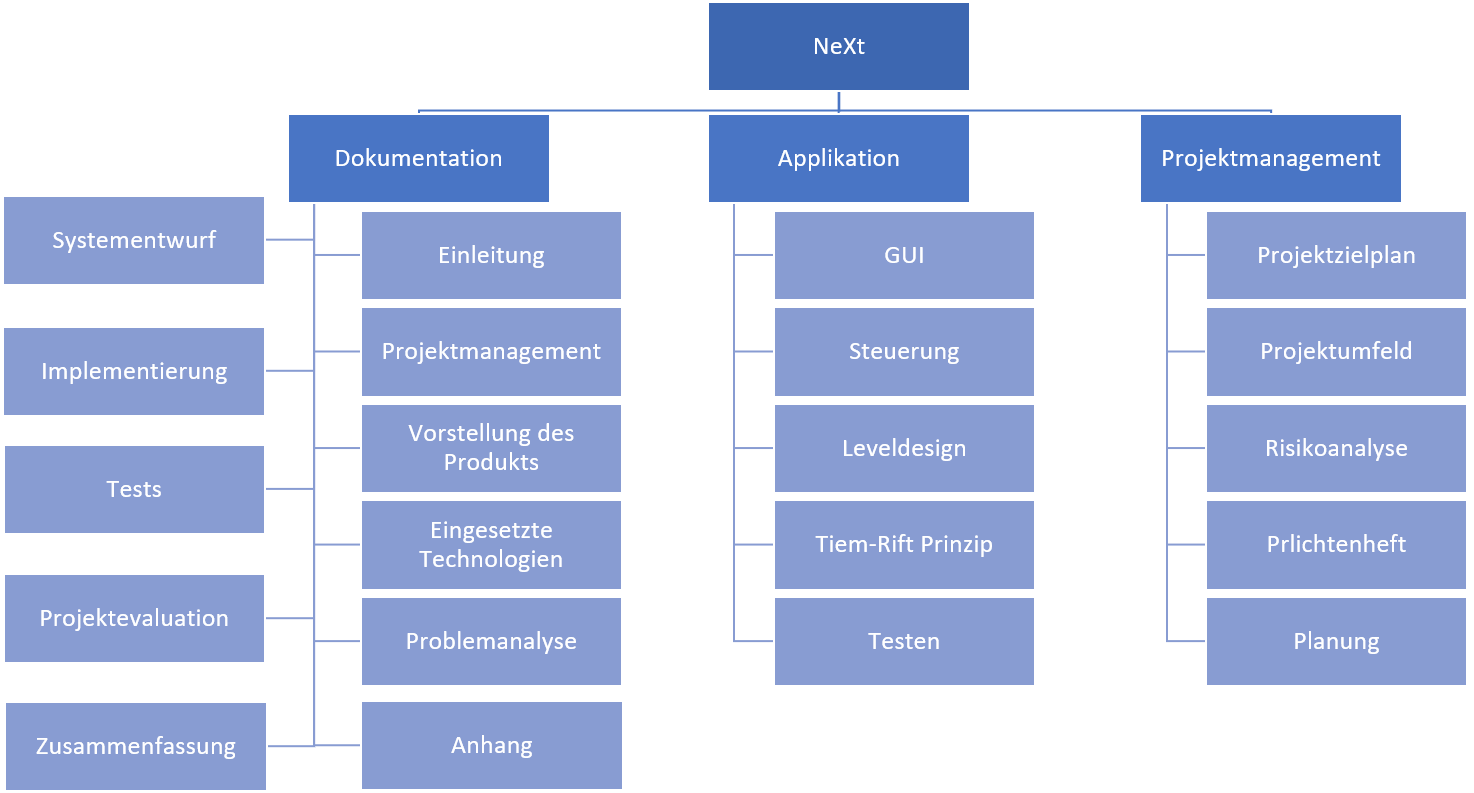
\includegraphics[width=16cm,height=8cm]{images/Projektstrukturplan.png}
	\captionbelow{Projektstrukturplan}
	\label{Projektstrukturplan}
\end{figure}

Der Projektstrukturplan, zu sehen in Abbildung \ref{Projektstrukturplan}, soll den gesamten Umfang des Projekts strukturiert und gut lesbar darstellen. Dabei ist zu erkenne, dass das Projekt aus drei großen Aufgabenbereichen besteht:
\begin{itemize}
	\item Dokumentation
	\item Applikation
	\item Projektmanagement
\end{itemize}
\def \currentAuthor {Lukas Vogel}
\newpage

\subsection{Meilensteine}
\def \currentAuthor {Michael Leitner}
\begin{itemize}
	\item 10.10.2017 Abschluss Anforderungsdefinition, Vorbereitung der Entwicklungsumgebung	
	\item 28.11.2017 Erster spielbarer Prototyp (Basissteuerung, Physik, Sound, Grafik, Test-Level)	
	\item 09.01.2018 spielbarer Prototyp nach dem Time Rift Prinzip	
	\item 06.02.2018 Erste spielbare Levels	
	\item 20.03.2018 vollständige Fertigstellung des Spiels mit einigen Levels, Beginn der Beta-Testing-Phase	
	\item 06.04.2018 Abschluss Beta-Testing	
	\item 30.04.2018 Verbesserung des Prototyps auf Basis der Rückmeldungen (Beta-Test)
	\item 15.06.2018 Fertigstellung der Dokumentation, Übergabe an den Auftraggeber
\end{itemize}
\subsection{Gantt-Chart}
\begin{figure}[H]
	\centering
	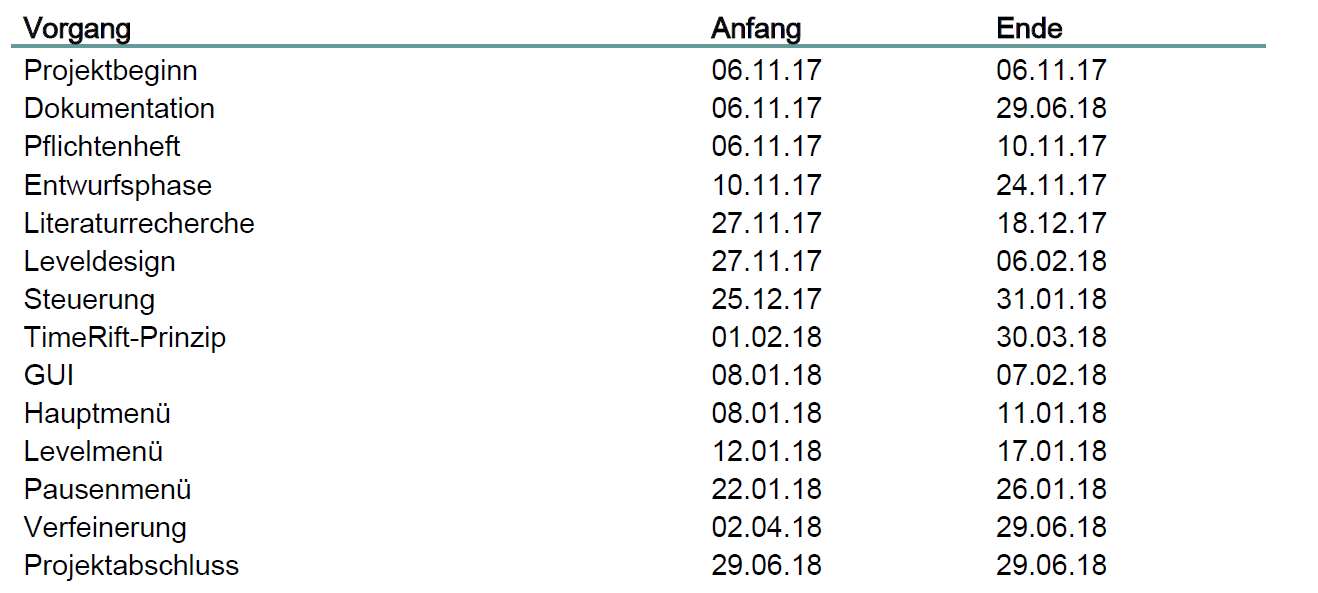
\includegraphics[width=15cm]{images/Vorgaenge.png}
	\caption{Vorgänge des Gantt Charts}	
	\label{Gantt-Auflistung}	
\end{figure}
In Abbildung \ref{Gantt-Auflistung} werden alle Vorgänge aufgelistet, die im Zeitmanagement aufgestellt wurden.

\begin{sidewaysfigure}
	\centering
	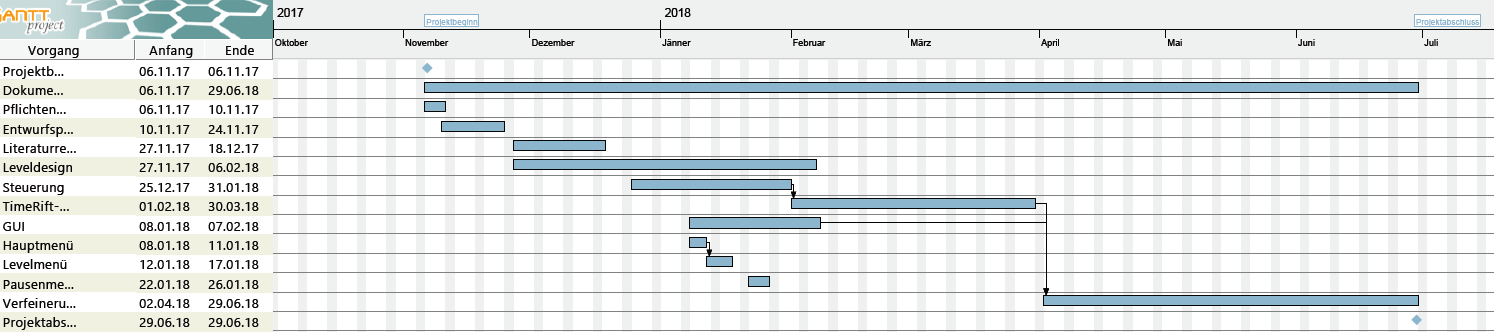
\includegraphics[width=20cm]{images/Gantt.png}
	\caption{Gantt Chart}
	\label{Gantt-Chart}
\end{sidewaysfigure}
Im nachfolgendem Gantt-Chart (Abb. \ref{Gantt-Chart}) sehen Sie, wie einzelne Vorgänge im Zusammenhang zu einander stehen. Eine Verzögerung bei dem Vorgang Steuerung würde eine Verzögerung bei Vorgang Time Rift bedeuten.
\chapter{Vorstellung des Produktes}
\section{Produktbeschreibung}
Das Computerspiel NeXt ist in den Genres Jump and Run und Puzzle angesiedelt. Hauptaugenmerk dieses Spiels ist das sogenannte Time Rift-Prinzip. Bei diesem Prinzip geht es darum, dass der Spieler jedes Level mehrmals in einzelnen Durchläufen spielen wird. Der Clue an der Sache ist jedoch, dass die zuvor gespielten Charaktere sich genauso bewegen wie sie in den vorigen Durchläufen gesteuert wurden. Das heißt: Hat der Spieler mit dem ersten Charakter einen Schalter betätigt, der eine Tür öffnet, dann wiederholt der Charakter diesen Vorgang, nur diesmal von selbst. Währenddessen kann der Spieler mit dem zweiten Charakter zu der zuvor genannten Tür gehen, welche sich öffnet, da der erste Charakter wieder den Schalter betätigt und somit wird das Level beendet. Durch dieses besondere Spielprinzip können vollkommen neue Puzzele-Elemente in das Produkt eingebaut werden, dies soll den Reiz des Spiels ausmachen. Damit das Spiel aber nicht zu leicht wird, wird noch ein Zeitfaktor eingebaut, welcher den Spieler unter Druck setzten soll. Schafft der Spieler es nicht den Schalter in der geforderten Zeit zu betätigen, so wird er mit dem zweiten Charakter nicht durch die Tür kommen und kann deshalb nicht das Level beenden. Durch ein abwechslungsreiches Level Design und das oben beschriebene Spielprinzip soll ein interessantes Spiel entwickelt werden, das auch einen großen Wiederspielfaktor als Ziel hat. Die Benutzeroberfläche so wie das Spielgefühl sollen intuitiv sein und für alle User keine große Umstellung zu anderen Spielen sein. Die genauen Mechaniken sowie die Funktionsweise des Spiels wurden in der Dokumentation erläutert.  
\chapter{Eingesetzte Technologien}
\def \currentAuthor {Lukas Vogel}
\section{Engine}

\subsection{Spiel-Engine}
Eine Spiel-Engine ist eine Art Framework, welches speziell für Computerspiele entwickelt wurde. Die Engine ist zuständig für den Spielverlauf aber auch für die visuelle Darstellung des Spielablaufs. Viele Spiel-Engines liefern eine Entwicklungsumgebung mit, diese liefert die Werkzeuge für die Entwicklung der jeweiligen Applikation mit.  \cite{Spiel-Engine}

\subsection{Unity-Engine}
Auf Anraten unseres Projektpartners verwendeten wir die Unity-Enigne, da das Unternehmen selbst damit arbeitet. Die Engine liefert eine Entwicklungsumgebung mit. Wir empfanden die Arbeit mit der Unity als angenehm. Zusätzlich ist es eine sehr weit verbreitete Spiel-Engine zu der es auch äußerst hilfreiches Lehrmaterial gibt. Unity selbst bietet auch eine Vielzahl an Lernvideos an.
Das Unternehmen Unity Technologies hat seinen Hauptsitz in San Francisco und wurde 2004 gegründet. Die Zielplattformen für Unity sind PCs, Spielkonsolen, mobile
Geräte sowie Webbrowser. 
 \cite{Unity-Engine}

\subsubsection{Technische Eigenschaften}
Nachstehend werden die wichtigsten technischen Eigenschaften der Unity-Engine erklärt. 

\textbf{Grafik}\\
Unity ist auf dem neusten Stand der Technik und unterstützt die verschiedensten Techniken, die derzeit in der Spielentwicklung benötigt werden. Außerdem können die eingebauten Beleuchtungseffekte selbst bearbeitet werden. Dies erweitert die Möglichkeiten der Engine nochmals signifikant.

\textbf{Animation}\\
Objekte des Spiels können über Skripte und andere Vorgehensweisen wie zum Beispiel physikalische Kräfte bewegt werden. Dieser Mechanismus war für unser Projekt sehr wichtig, da der Spieler die Charaktere selbst in Echtzeit steuert.

\textbf{Programmierung}\\
Unity unterstützt drei verschiedene Programmiersprachen:
\begin{itemize}
	\item C\#
	\item UnityScript (vergleichbar mit JavaScript)
	\item Boo
\end{itemize}
Diese sind notwendig um Skripte zu erstellen, welche die von Unity eingebauten Mechanismen erweitern. Da wir im Unterricht bereits mit C\# Erfahrungen sammeln konnten, haben wir diese verwendet.

\textbf{Werkzeuge}\\
Die Engine ist mittels Werkzeugen erweiterbar, diese sind zu einem Teil kostenlos verfügbar und als einfache Plug-ins zu integrieren. Bei unserem Projekt konnten wir dadurch ohne Kosten einfache Grafiken und nützliche Tools einsetzen.\\
\cite{Unity-Engine}

\section{Entwicklungsumgebung}
\subsection{Unity-Editor}
Als Entwicklungsumgebung wählten wir Unity-Editor da sie vom selben Unternehmen entwickelt wurde und somit speziell für die Unity-Engine gemacht wurde. Sie wurde basierend auf gängigen 3D-Animationsprogrammen designet. Sie ist sehr einfach zu bedienen und ermöglicht das importieren von Werkzeugen mittels eines einfachen Mausklicks. In dieser Entwicklungsumgebung können alle für die Spielentwicklung wichtigen Arbeiten verrichtet werden. Für das Programmieren der Scripte verwendeten jedoch wir Visual Studio.  \cite{Unity-Engine}

\subsection{Visual Studio}
Wir verwendeten für die Programmierung von Scripten Visual Studio Community 2017, welche für Studenten kostenlos ist und wir im Unterricht zum Entwickeln von Apllikatione mit C\# verwendeten. 

\section{C\#}
Im Unterricht hatten wir unseren ersten Kontakt mit der Programmiersprache C\#. Bei diesem Projekt konnten wir unser erlerntes Wissen nutzen, da wir es für die Scripte in Unity verwendeten.

\section{Dokumentation}
Für die Dokumentation der Diplomarbeit verwendeten wir auf Anraten von unserem Betreuer LaTeX in Kombination mit der Applikation TeXstudio. LaTeX vereinfacht
Verantwortlich für den Inhalt: Lukas Vogel	Seite 35 die Benutzung von TeX einem Textsatzsystem mittels Makros. TeXstudio ist eine Entwicklungsumgebung, die für LaTeX entwickelt wurde.
 \cite{Latex}
\chapter{Problemanalyse}
\section{USE-Case-Analyse}
\def \currentAuthor {Lukas Vogel}
In diesem Projekt wurde eine USE-Case-Analyse vollzogen. Als Benutzer gibt es nur den Anwender der Applikation. Nachstehend sind zwei Anwendungsfälle mittels Use-Case-Diagrammen beschrieben worden
\subsection{Anwendungsfall: Level starten}
Damit man das Computerspiel spielen kann muss zuerst ein Level ausgewählt werden. Dies wird über die verschiedenen Menüs bewerkstelligt. In Abbildung \ref{USE-Case-Menu} ist dieser Anwendungsfall als Diagramm dargestellt worden. 
\begin{figure}[H]
	\centering
	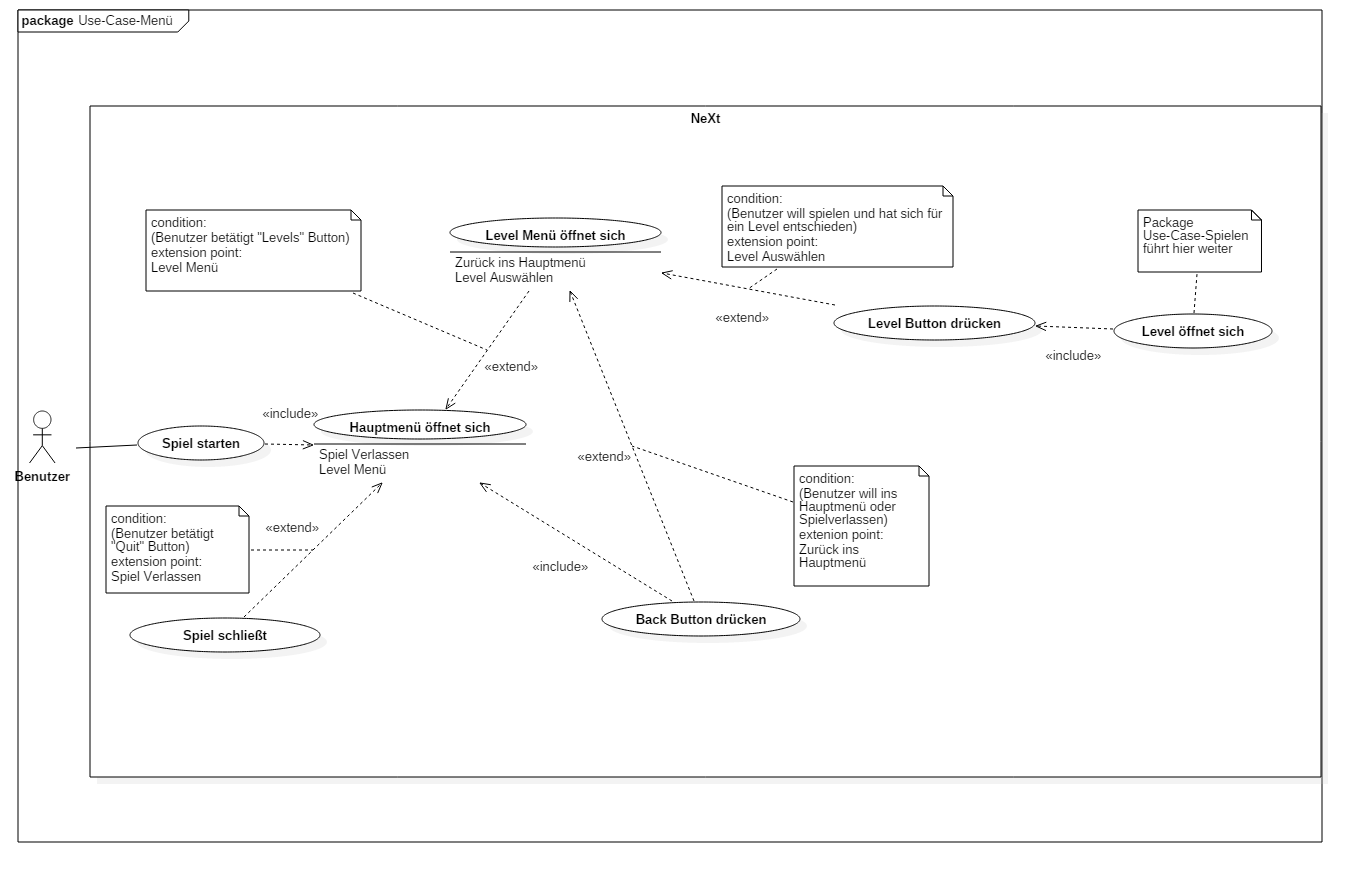
\includegraphics[angle=90,scale=0.45]{images/UseCaseMenu.png}
	\caption{USE-Case-Menü}
	\label{USE-Case-Menu}
\end{figure}
\subsection{Anwendungsfall: Spielen}
Sobald ein Level ausgewählt wurde kann mit dem Spielen begonnen werden. Der Verlauf eines Levels wird mit dem Diagramm, welches in Abb. \ref{USE-Case-Spielen} zu sehen ist, beschrieben. Des Weiteren ist das Time Rift Prinzip sehr gut zu erkennen.
\begin{figure}[H]
	\centering
	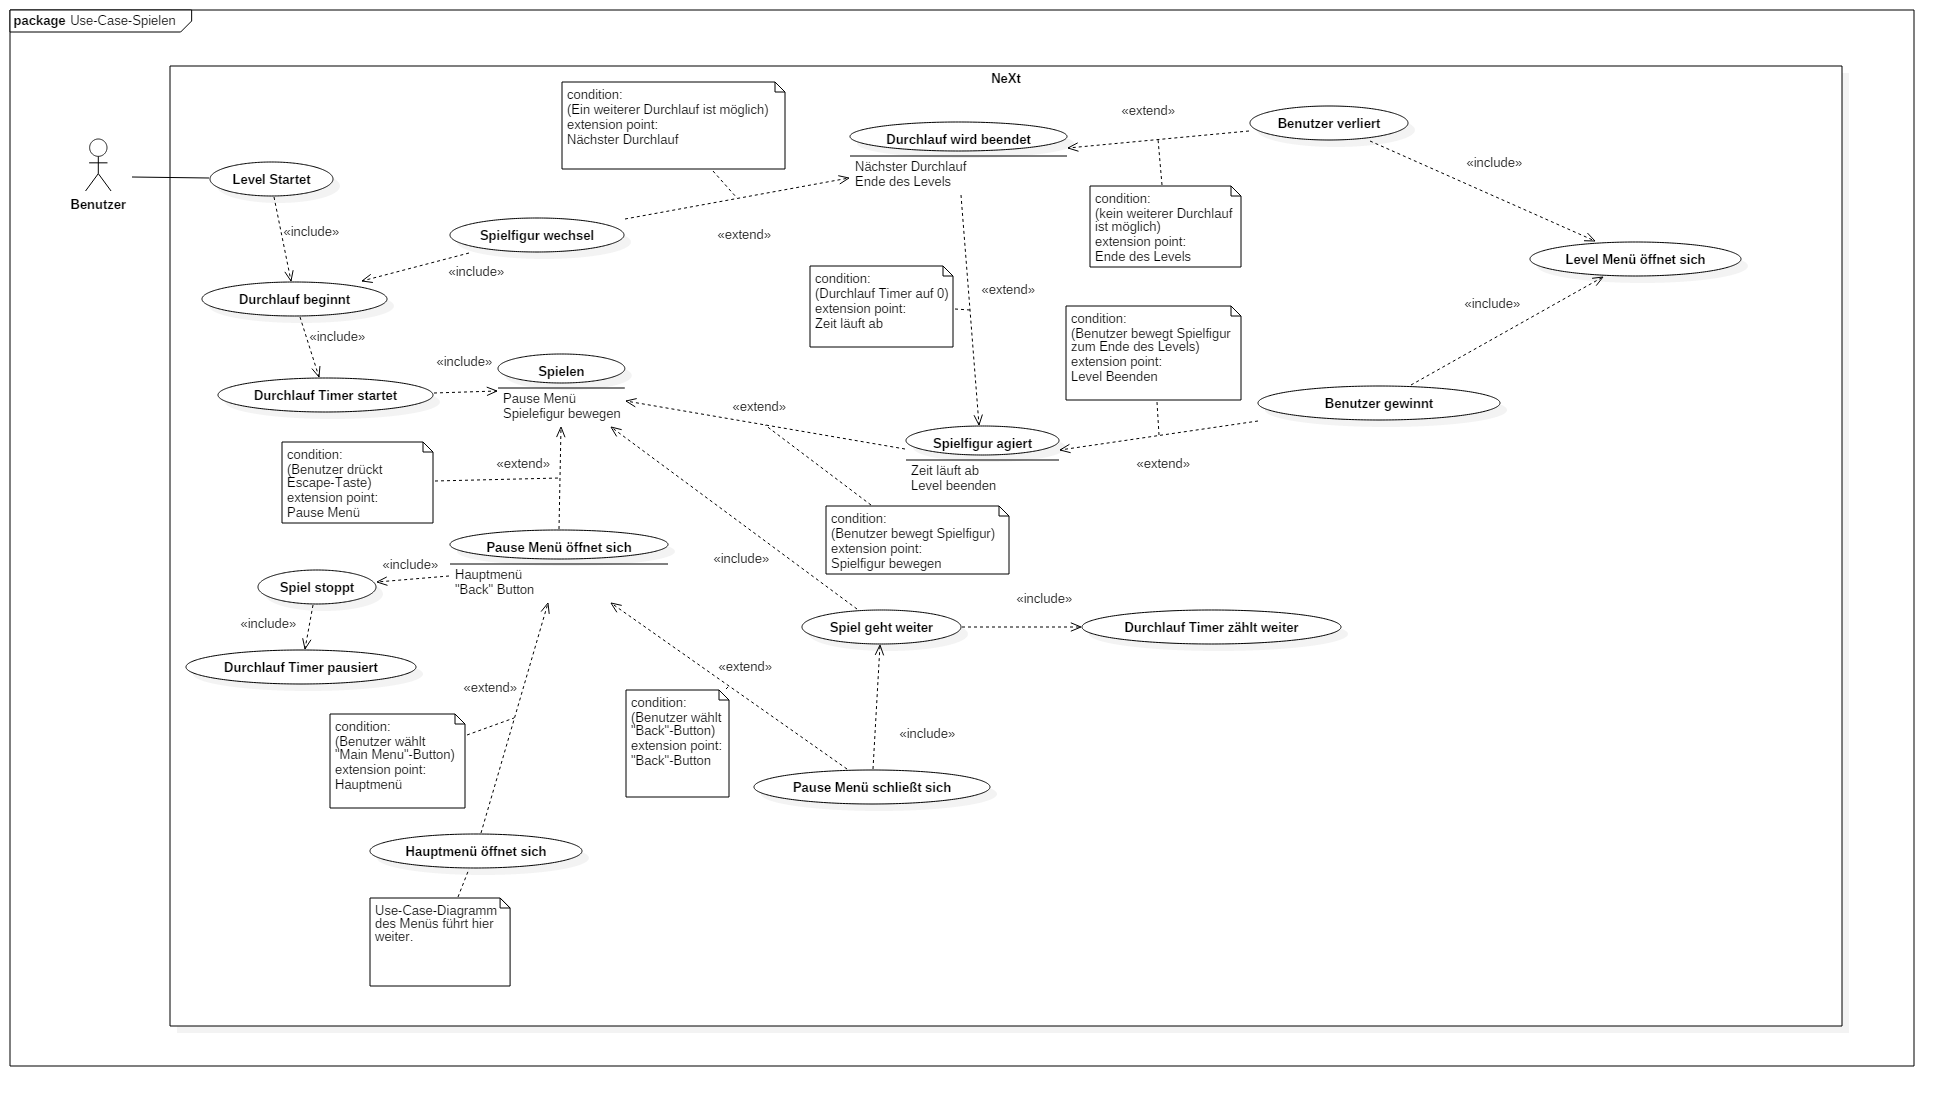
\includegraphics[angle=90,scale=0.30]{images/UseCaseSpielen.png}
	\caption{USE-Case-Spielen}
	\label{USE-Case-Spielen}
\end{figure}
\section{User-Interface-Design}
5.2.	User-Interface-Design
Im folgenden Teil der Dokumentation sind verschiedene Wireframes der Benutzeroberfläche des Programms zu sehen.

\begin{figure}[H]
	\centering
	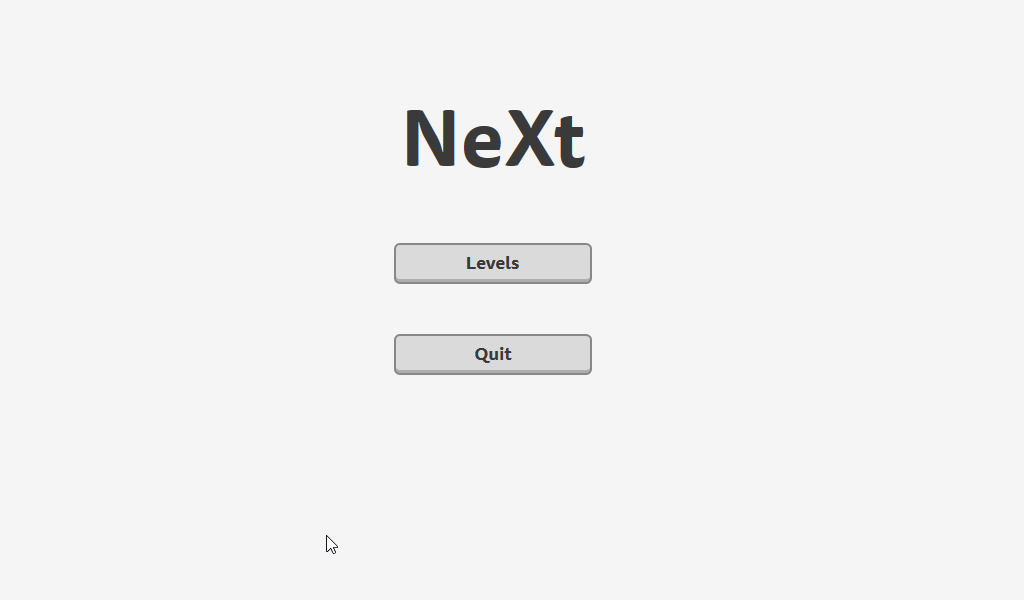
\includegraphics[width=16cm, height=9cm]{images/WireframeMainmenu.png}
	\caption{Wireframe-Hauptmenü}
	\label{WireframeMainmenu}
\end{figure}
In Abbildung \ref{WireframeMainmenu} ist der erste Entwurf für das Hauptmenü des Spiels zu sehen. Diese Ansicht ist die erste, die der Benutzer sehen soll, wenn er das Computerspiel startet. Das Menü ist sehr einfach gehalten. Es gibt ein Textfeld welches ’NeXt’ anzeigt und darunter zwei Buttons. Der obere Button soll den Spieler in das Menü der Levels leiten, siehe Abbildung \ref{WireframeLevelsmenu}. Der untere Button soll die Applikation schließen.

\begin{figure}[H]
	\centering
	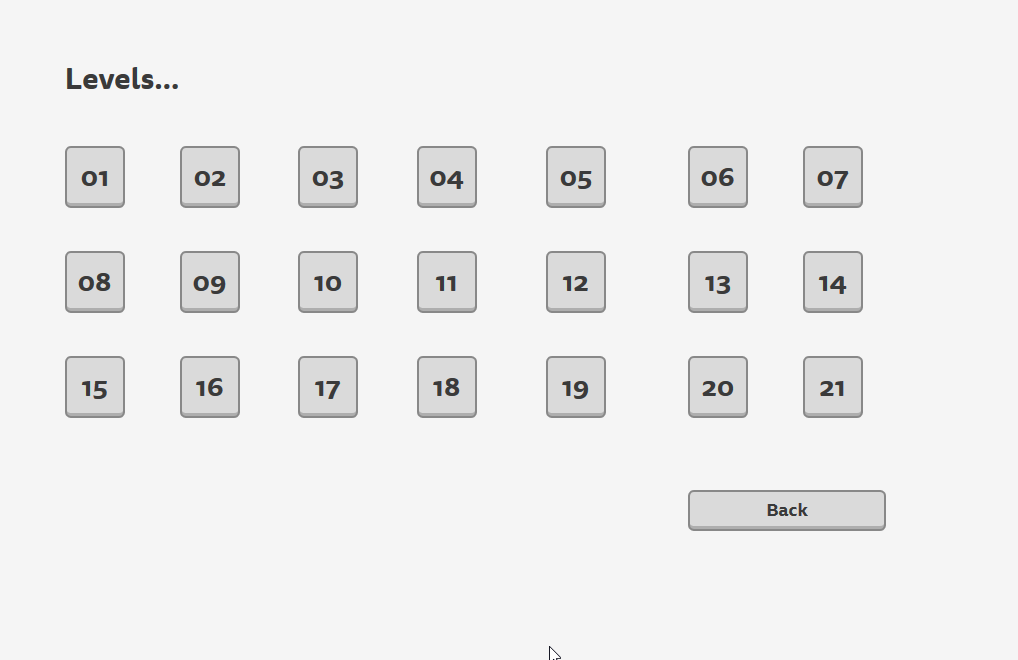
\includegraphics[width=16cm, height=9cm]{images/WireframeLevelsmenu.png}
	\caption{Wireframe-Levelmenü}
	\label{WireframeLevelsmenu}
\end{figure}
Das nächste Wireframe in Abbildung \ref{WireframeLevelsmenu} zeigt eine Übersicht aller spielbaren Levels welche als nummerierte Buttons dargestellt werden. Wenn der Benutzer einen Level-Button betätigt soll sofort das gewählte Level starten. Der Button rechts unten mit der Beschriftung ’Back’ soll den Spieler wieder zurück in das Hauptmenü führen.

\begin{figure}[H]
	\centering
	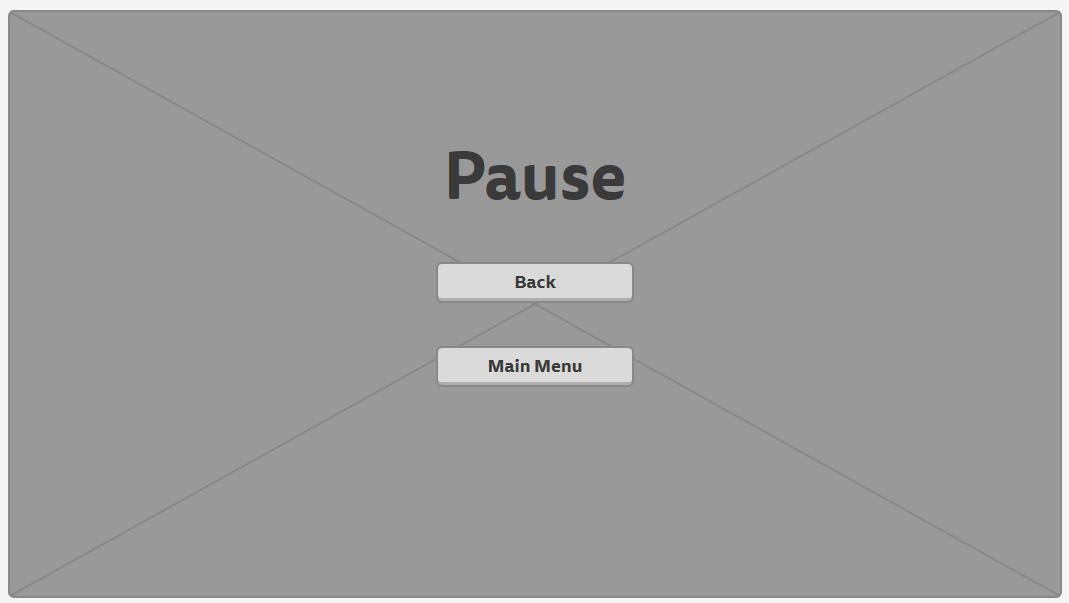
\includegraphics[width=16cm, height=9cm]{images/WireframePausemenu.png}
	\caption{Wireframe-Pausemenü}
	\label{WireframePausemenu}
\end{figure}
Sobald der Benutzer sich in einem Level befindet soll er die Möglichkeit haben, mittels Escape-Taste das Spiel zu stoppen und in das Pause-Menü zu wechseln. Das Wireframe dazu ist in Abbildung \ref{WireframePausemenu} zu sehen. Die graue Fläche soll dabei das Level darstellen, welches im Hintergrund immer noch zu sehen sein soll. Zusätzlich sind noch zwei Buttons zu sehen. Der erste Button mit dem Text ’Back’ soll das Menü wieder schließen und das Spiel weiterlaufen lassen. Der Zweite, welcher mit der Beschriftung ’Main Menu’ versehen ist, soll denn Benutzer wieder in die Ansicht des Hauptmenüs, Abbildung \ref{WireframeMainmenu} bringen.

\chapter{Systementwurf}

\section{Architektur}
\def \currentAuthor {Michael Leitner}
In der Unity3D Entwicklungsumgebung werden keine klassischen Architekturmuster verwendet. Wenn ein bestimmtes Objekt ein Skript benötigt, wird ihm dieses Skript angehängt. Jedoch wurden für das Time Rift-Prinzip mehrere Klassen verwendet.


\begin{figure}[H]
	\centering
	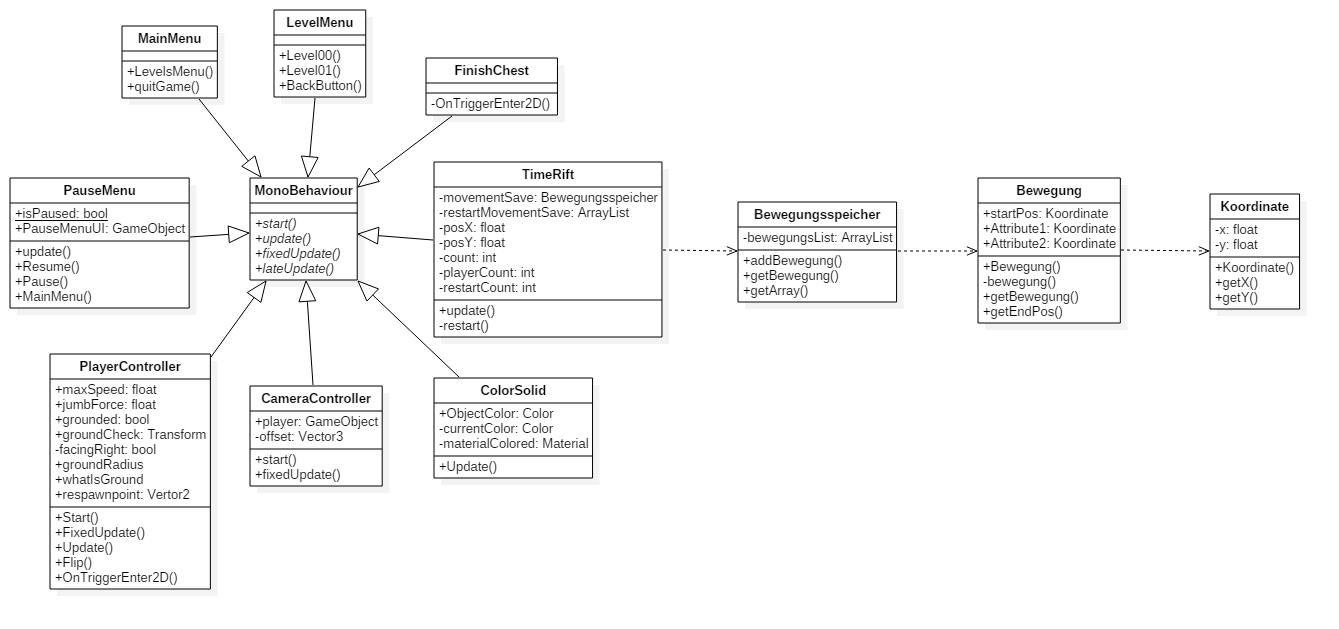
\includegraphics[width=15cm]{images/UML.png}
	\caption{UML-Diagramm der Klassen}		
\end{figure}

Wie man aus dem UML Diagramm sehen kann, erben alle Spielablaufs bezogenen Klassen von MonoBehaviour, genaueres dazu können Sie bei Punkt \ref{MonoBehaviour}

\chapter{Implementierung}
\section{Unity-Klassenstruktur}
\subsection{MonoBehaviour}	\label{MonoBehaviour}
Die Klasse „MonoBehaviour“ ist eine Standardklasse, die von der Unity3D-Engine bereitgestellt wird. Jedes Skript, welches in Unity verwendet wird, muss von dieser Klasse erben (Ähnlich wie in Java die „Object-Klasse“ von jeder Klasse gerbt wird). MonoBehaviour gibt folgende Methoden zur Verfügung:
\begin{itemize}
	\item Start()
	\item Update()
	\item FixedUpdate()
	\item LateUpdate()
	\item OnGUI()
	\item OnDisable()
	\item OnEnable()
\end{itemize}
Verwendet werden in diesem Projekt aber nur die Start, Update, FixedUpdate und LateUpdate Methoden.
\subsubsection{Start-Methode}
Die Start-Methode wird nur einmal in der Skriptlaufzeit aufgerufen und zwar bei der Initialisierung des Skriptes.
\subsubsection{Update-Methode}
Die Update-Methode wird bei jedem Frame aufgerufen. Sie wird meistens für Berechnungen, die in jedem Frame durchgeführt werden müssen, verwendet. Nachteil hier ist aber, wenn das Spiel eine schlechte Framezahl hat werden die Berechnungen auch weniger oft durchgeführt.
\subsubsection{FixedUpdate-Methode}
Die FixedUpdate-Methode wird bei jedem fixierten Framerate Frame aufgerufen. Diese Methode soll verwendet werden für Bewegungen eines Charakters (spielbar und nicht spielbar). Dies hat den Grund, dass selbst bei schlechter Framerate, die Berechnungen der Bewegung konstant bleiben.
\subsubsection{LateUpdate-Methode}
Die LateUpdate-Methode wird nach allen anderen Update-Methoden aufgerufen. Sie wird hauptsächlich für Funktionen verwendet die nach all den Update-Methoden aufgerufen werden soll z.b.: Für die Kameraführung, da sich Objekte in der UpdateMethode bewegt haben können.
\subsection{Weitere bereitgestellten Funktionen}
Unity stellt ebenso wichtige Funktionen für die Spielentwicklung bereit, unter anderem wird Physik und Kollisionen bereits von Unity bereitgestellt, müssen aber vom Entwickler auf seinen Wunsch angepasst werden. Auch für die Bewegungsberechnungen wird von Unity schon viel bereitgestellt. Zum Beispiel die "Vector2"- Funktion. Diese Funktion beschreibt wie man einen 2-Dimensionalen Vektor berechnet. 

\section{GUI}
\def \currentAuthor {Lukas Vogel}
Das Graphical User Interface des Spiels wurde sehr einfach gehalten, da es sich um eine Prototyp handelt.
\subsection{Hauptmenü}
Das Hauptmenü besteht aus einem Text und zwei Buttons, zu sehen in Abb.\ref{Mainmenu}. Damit das Menü das gezeigte Aussehen hat sind folgende Arbeitsschritte zu machen:

\begin{figure}[H]
	\centering
	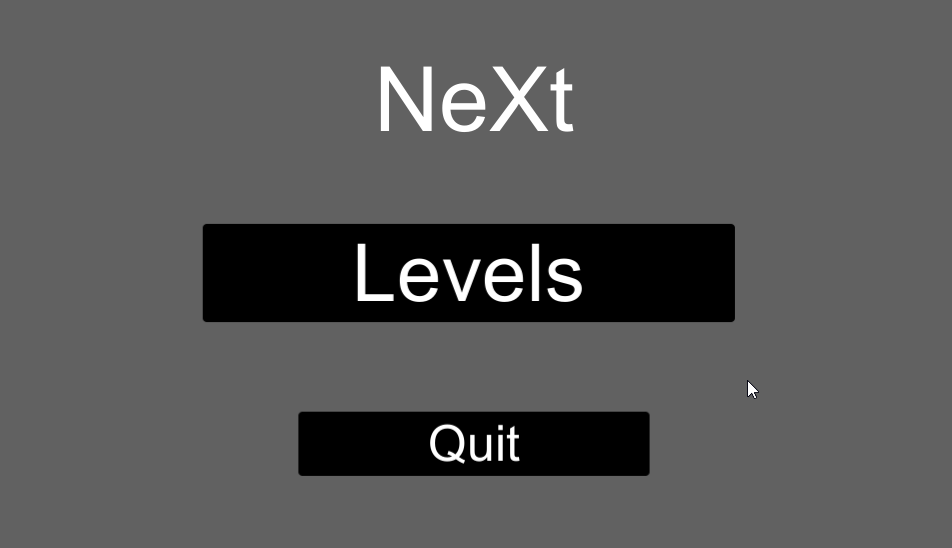
\includegraphics[height=8cm]{images/Mainmenu.png}
	\caption{Hauptmenü}
	\label{Mainmenu}
\end{figure}
Als erstes wird eine leere Szene benötigt. Dafür kann einfach die Tastenkombination Strg. + C gedrückt werden oder unter dem Menü links oben von Unity-Editor File –> New Scene.

Wenn die neue Szene angelegt ist, mittels Rechtsklick in der Hierarchie der Szene, ein neues Panel-Objekt anlegen, Abbildung \ref{PanelAnlegen}. Durch das Anlegen eines Panels wird auch automatisch ein Canvas-Objekt erstellt, welches hierarchisch gesehen über dem Panel steht.

\begin{figure}[H]

	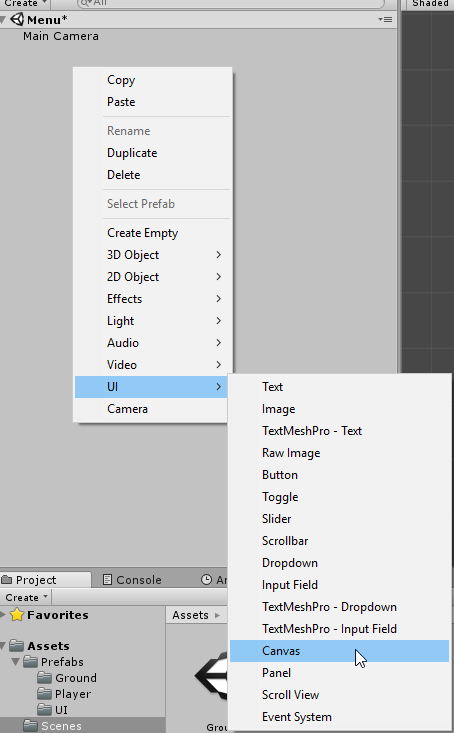
\includegraphics[height=8cm]{images/PanelAnlegen.png}
	\caption{Anlegen eines Panel-Objekts}
	\label{PanelAnlegen}
\end{figure}
Bei dem Canvas-Objekt müssen die Einstellungen von Abb. \ref{CanvasSetup} getroffen werden damit es das gewünschte verhalten erbringt.
\begin{figure}[H]
	\centering
	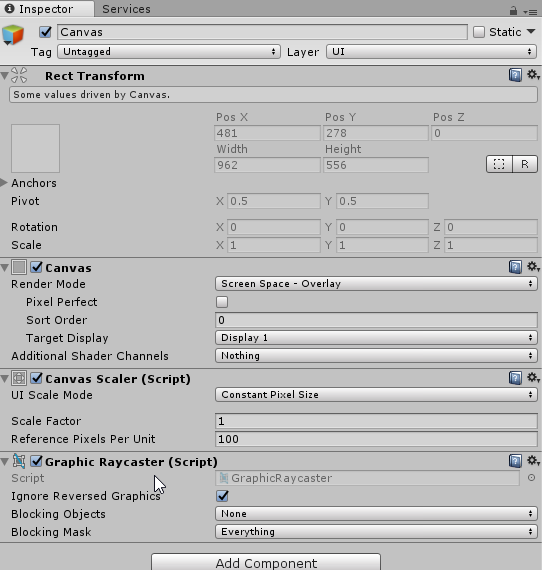
\includegraphics[height=8cm]{images/CanvasSetup.png}
	\caption{Einstellung des Canvas-Objekts im Hauptmenü}
	\label{CanvasSetup}
\end{figure}
Wenn diese Einstellungen alle übereinstimmen ist der nächste Schritt das Bearbeiten des Panels. Hier muss als erstes die Hintergrundfarbe des Menüs festgelegt werden. Dies ist möglich bei der Komponente ’Image’. Wahlweise kann nun eine Grafik für das Attribut ’Source Image’ gewählt werden oder man verwendet nur eine Farbe, wie in unserem Fall, um den Hintergrund des Menüs darzustellen. Darüber hinaus wäre es noch möglich einen speziellen Effekt beim Hintergrund zu erzielen, mittels der ’Material’ Eigenschaft. Alle Eigenschaften für das Panel-Objekt sind in Abbildung \ref{PanelSetup} zu sehen.
\begin{figure}[H]
	\centering
	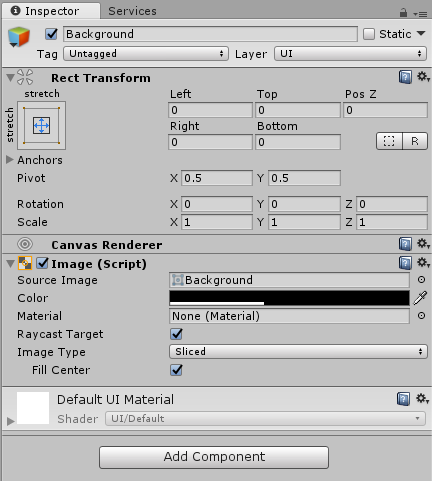
\includegraphics[height=8cm]{images/PanelSetup.png}
	\caption{Einstellung des Panel-Objekts im Hauptmenü}
	\label{PanelSetup}
\end{figure}
Sobald das Panel-Objekt fertig konfiguriert ist geht es an den nächsten Arbeitsschritt. Als Erstes wird ein Textfeld erstellt welches mittels Rechtsklick in der Hierarchie links, unter dem UI zu finden ist.
Das Textfeld ist ein einfach aufgebautes Objekt. Hier wurde lediglich der Text ’NeXt’ beim Attribut Text angegeben und die Schriftgröße auf 30 erhöht, zu sehen in Abbildung  \ref{TextSetupMainMenu}
\begin{figure}[H]
	\centering
	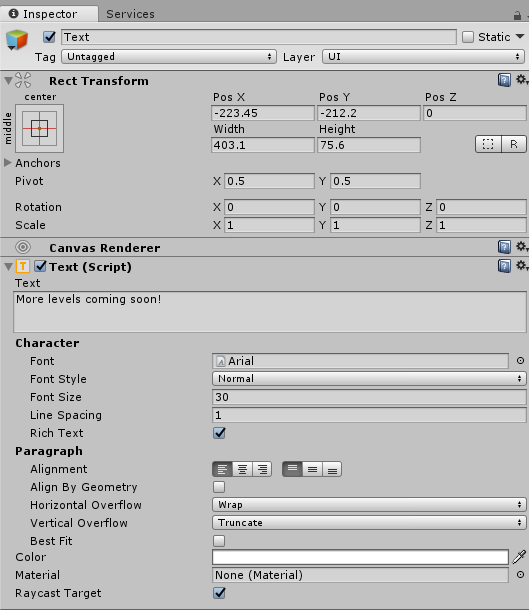
\includegraphics[height=8cm]{images/MainMenuTextSetup.png}
	\caption{Einstellungen des Text-Objekts im Hauptmenü}
	\label{TextSetupMainMenu}
\end{figure}
 Daraufhin wurden die Buttons, wie die vorigen Objekte, hinzugefügt. Der Button, welcher später zum Level-Menü führt, wurde bewusst größer gemacht als der ’Quit’-Button, der das Spiel schließt, da so dem Spieler die Auswahl der Levels besser ins Auge sticht. Ein Button-Objekt hat in der Hierarchie unter sich immer ein TextObjekt, wenn es neu erstellt wird. Dieses Textfeld ist die Beschriftung des Buttons. Da wir uns für einen grauen Hintergrund entschieden wurde der Text der Buttons weiß. Die Buttons selbst haben, je nach Position des Mauszeigers, verschiedene Farben. Für das Attribut ’Normal Color’ wählten wir schwarz und wenn der Button gedrückt wird ändert sich seine Farbe auf ein dunkles Grau (Attribut: ’Pressed Color’). Dieses verhalten wird in Abbildung \ref{ButtonClicked} veranschaulicht.
 
  \begin{figure}[H]
  	\centering
  	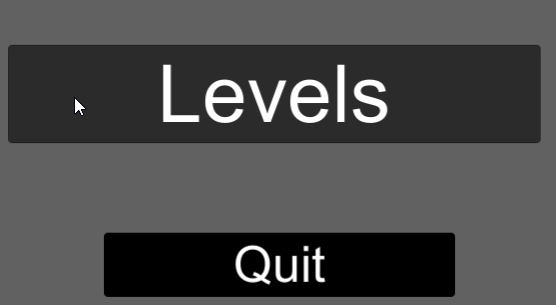
\includegraphics[width=10cm]{images/ButtonsClicked.png}
  	\caption{Farbwechsel des Buttons im Hauptmenü beim Klicken}
  	\label{ButtonClicked}
  \end{figure}


Ist das Einrichten soweit erreicht, geht es darum das Verhalten der Buttons bei einem Click-Event zu steuern. Damit für jeden Button nicht extra ein Skript erstellt werden muss, erstellen wir als erstes ein sogenanntes ’Empty Objekt’ welches, wie der Name schon sagt, leer ist. Danach werden die beiden Buttons in der Hierarchie unter das neu generierte Objekt gestellt. Dieser Schritt ist in Abb. \ref{MainMenuEmpty} zu sehen wobei ’MainMenu’ das Empty-Objekt, ’Background’ das Panel-Objekt und ’LevelsButton’ sowie ’QuitButton’ die Button-Objekte darstellt.

\begin{figure}[H]
	\includegraphics[width=4cm]{images/MainMenuEmpty.png}
	\caption{Teil der Hierarchie des UI im Hauptmenü.}
	\label{MainMenuEmpty}
\end{figure}
Nun wurde ein neues Skript im gewünschten Ordner angelegt. Bei uns hat dieser den Namen ’Script’. In der Projektstruktur unten einfach mittels Rechtsklick ein C\# Skript anlegen (Abbildung \ref{addScript}). Sobald es erstellt ist, muss es nur noch Programm Code hinein.

\begin{figure}[H]
	\includegraphics[height=8cm]{images/addScript.png}
	\caption{Anlegen eines C\# Scripts im Unity-Editor}
	\label{addScript}
\end{figure}

Im Script 'MainMenu' ist der folgende (\cref{code:MaineMenuScript}) Code Enthalten.

\begin{lstlisting}[language={[Sharp]C}, caption=MainMenu-Script, label=code:MaineMenuScript]
using System.Collections;
using System.Collections.Generic;
using UnityEngine;
using UnityEngine.SceneManagement;

public class MainMenu : MonoBehaviour {

public void LevelsMenu()
{
SceneManager.LoadScene(1);
}

public void quitGame()
{

Application.Quit();
}
}

\end{lstlisting}
Die Methode ’LevelsMenu’ wechselt die Szene vom Hauptmenü des Spiels zur Szene ’LevelMenu’. Dies wird mit der Methode ’Load Scene(1)’ gemacht. Die Zahl 1, die als Parameter mit gegeben wird, steht für den Index des Levels Menüs welcher in den ’Build Settings’ (Abb. \ref{BuildSettings}) festgelegt werden kann. Die Methode ’quitGame()’ schließt die gesamte Applikation.
\begin{figure}[H]
	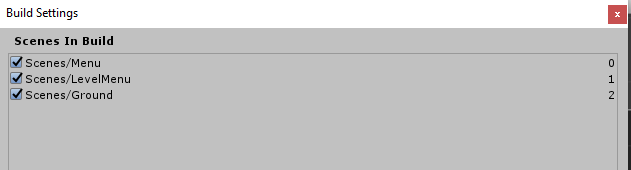
\includegraphics[width=10cm]{images/BuildSettings.png}
	\caption{Ausschnitt der Build Settings des Unity-Editors}
	\label{BuildSettings}
\end{figure}
Ist das Skript abgespeichert, wird es als Erstes dem Empty-Objekt als Komponente hinzugefügt, danach können nun die einzelnen Methoden den jeweiligen Buttons zugewiesen werden. Dafür im Inspector des Buttons in der Komponente ’Button’ nach ’on Click()’ suchen. Als Objekt muss nun das Script ’MainMenu’ angegeben und die passende Methode ausgewählt werden, zu sehen in Abbildung \ref{onClick}. Damit wäre das Hauptmenü komplett implementiert.
\begin{figure}[H]
	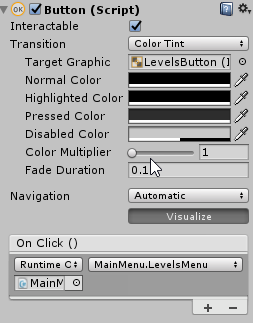
\includegraphics[height=8cm]{images/ButtonScriptLevelsButton.png}
	\caption{Einstellungen der 'Button' Komponente für den Levels-Button im Hauptmenü}
	\label{onClick}
\end{figure}
\subsection{Level-Menü}
Nun da das Hauptmenü abgeschlossen ist kann das Level-Menü entwickelt werden. Dieses zeigt alle vorhandenen Levels an und ermöglicht es, sie zu starten.
Auch hier wird als Erstes wieder ein Panel-Objekt erstellt, welches den Hintergrund der Szene darstellt. Sobald dies erledigt ist, wird ein Text-Objekt, welches die Überschrift der Szene mit dem Text ’Levels’ erstellt und in die linke obere Ecke gesetzt. Nun werden die Buttons erzeugt, als erstes jene für die jeweiligen Levels. Die Buttons für die Level haben die Maße eines Quadrats bekommen, in ihnen wird lediglich die Zahl, die das jeweilige Level repräsentiert gezeigt (zum Beispiel: 01). Die Buttons verhalten sich vom Farbwechsel her genau wie die des Hauptmenüs. Insgesamt wurden vier dieser Level-Buttons erstellt. Des Weiteren ist es noch wichtig dem Benutzer eine Möglichkeit zu bieten wieder zurück ins Hauptmenü zu gelangen. Dies wurde mittels eines ’Back-Buttons’ realisiert. Dieser wurde den Buttons, in Form und Verhalten der Buttons, des Hauptmenüs nachempfunden. Zu guter Letzt wurde noch ein Textfeld erstellt, dass den Benutzer darauf hinweist das noch weitere Levels in Zukunft kommen werden. Das fertige Level-Menü ist in Abbildung \ref{Levelmenu} veranschaulicht.


\begin{figure}[H]
	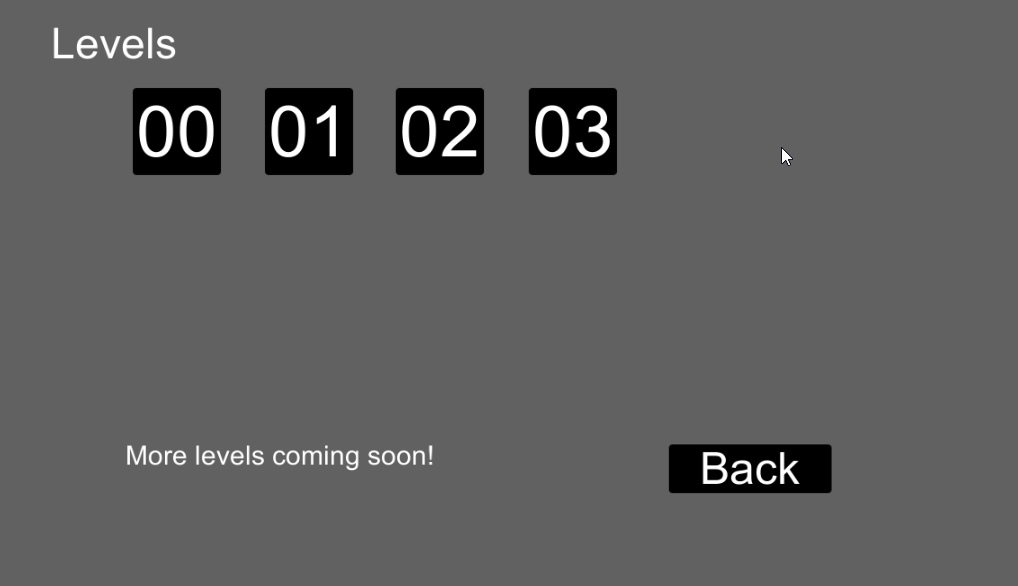
\includegraphics[height=8cm]{images/Levelmenu.png}
	\caption{Level-Menü}
	\label{Levelmenu}
\end{figure}

Damit die Buttons auch funktionieren wird zuerst ein Empty-Objekt erstellt und alle Buttons werden ihm hierarchisch untergeordnet. Das Skript wird wiederum dem Empty-Objekt als Komponente zugewiesen. Der Codes des Skripts ist in Listing \cref{code:LevelMenu-Skript}

\begin{lstlisting}[language={[Sharp]C}, caption=LevelMenu-Script, label=code:LevelMenu-Skript]
using System.Collections;
using System.Collections.Generic;
using UnityEngine;
using UnityEngine.SceneManagement;

public class LevelMenu : MonoBehaviour {

public void Level00()
{
SceneManager.LoadScene(2);
}

public void Level01()
{
SceneManager.LoadScene(1);
}

public void Level02()
{
SceneManager.LoadScene(3);
}

public void Level03()
{
SceneManager.LoadScene(4);
}
public void BackButton()
{
SceneManager.LoadScene(0);
}

}
\end{lstlisting}
Die in \cref{code:LevelMenu-Skript} gezeigten Methoden verwenden alle die Methode ’LoadScene()’ der Unterschied zwischen ihnen liegt jedoch darin, dass jede von ihnen auf eine andere Szene leitet.

\subsection{Pause-Menü}
Damit der Benutzer auch innerhalb eines Levels das Spiel beenden oder auch stoppen kann wurde das Pause Menü entwickelt. Es funktioniert in jedem Level exakt gleich, deswegen wird es nur einmal beschrieben.
Der Spieler soll durch das Betätigen der Escape-Taste das Spiel anhalten können, sodass sich die Spielfigur nicht mehr bewegt. Zusätzlich soll er die Optionen haben das Spiel wieder fortzuführen oder zurück ins Hauptmenü zu gelangen.
Als Erstes wird ein Canvas-Objekt im jeweiligen Level erstellt. Im ’Inspector’ rechts muss sichergestellt werden, dass bei der Komponente ’Canvas’ im Canvas-Objekt die Eigenschaft ’Render Mode’ auf ’Screen Space - Overlay’ gesetzt wird und bei ’Pixel Perfect’ der Hacken gesetzt ist, zu sehen in Abbildung \ref{CanvasPause}.


\begin{figure}[H]
	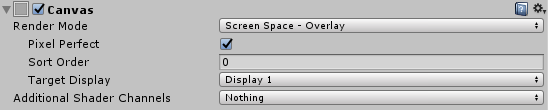
\includegraphics[width=10cm]{images/CanvasPause.png}
	\caption{Einstellungen des Canvas-Objekts bei der Canvas-Komponente}
	\label{CanvasPause}
\end{figure}

Danach wird ein Panel-Objekt erzeugt dessen Farbe auf ein transparentes Schwarz und die Eigenschaft ’Source Image’ auf ’None’ bei der ’Image’-Komponente gesetzt wird zu sehen in Abbildung \ref{Panel Pause}

\begin{figure}[H]
	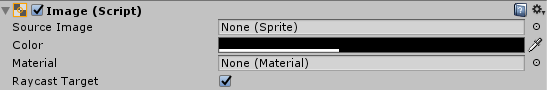
\includegraphics[width=10cm]{images/PanelPause.png}
	\caption{Einstellungen des Panel-Objekts bei der 'Image'-Komponente}
	\label{Panel Pause}
\end{figure}

Der nächste Arbeitsschritt ist es eine Überschrift für das Menü zu erstellen. Der Text lautet ’Pause’, die Schriftgröße wird angepasst und er soll dieses mal einen Schatten bekommen. Dafür wird dem Objekt die Komponente ’Shadow’ hinzugefügt, siehe Abbildung \ref{addshadow}.

\begin{figure}[H]
	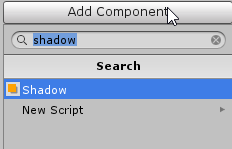
\includegraphics[width=6cm]{images/addshadow.png}
	\caption{Hinzufügen der 'Shadwo'-Komponente}
	\label{addshadow}
\end{figure}

Nachdem die Komponente ergänzt wurde, wird dessen Eigenschaft ’Effect Distance’ beim X-Wert auf 4 und beim Y-Wert auf -4 eingestellt (Abb. \ref{shadowSetup}). Damit wäre dieser Teil des Menüs abgeschlossen.
\begin{figure}[H]
	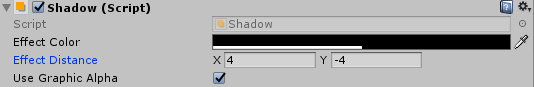
\includegraphics[width=10cm]{images/shadowSetup.png}
	\caption{Einstellungen der 'Shadwo'-Komponente}
	\label{shadowSetup}
\end{figure}

Nun kommen die Buttons dran. Es werden zwei Buttons erstellt. Ein ’Back’-Button und ein ’Main Menu’-Button.
Im Pause-Menü werden jedoch nicht die bisher verwendeten Buttons wiederverwendet. Da das Spiel im Hintergrund des Menüs zu sehen ist soll, der Rahmen sowie dessen Füllung transparent sein. Falls jedoch der Spieler mit der Maus über einen fährt, soll dieser wieder schwach erkennbar sein und wenn der Button betätigt wird soll dessen Sichtbarkeit noch stärker sein. Des Weiteren bekommt auch die Schrift der Buttons eine ’Shadow’-Komponente mit denselben Einstellungen wie bei der
Überschrift.
Damit die Transparenz der Buttons sich so verhält wie gewünscht, wird der Alpha Wert der Farben ’Normal Color’, ’Highlighted Color’, sowie ’Pressend Button’ angepasst. Das heißt bei ’Normal Color’ auf den Wert 0 und bei den anderen Beiden auf 100 und 200.
Da das Menü nicht durchgehend zu sehen sein soll, wird das Panel-Objekt deaktiviert, dies ist mittels eines einfachen Mausklicks zu bewerkstelligen, siehe Abbildung \ref{deactivatePanel}, rote Markierung.

\begin{figure}[H]
	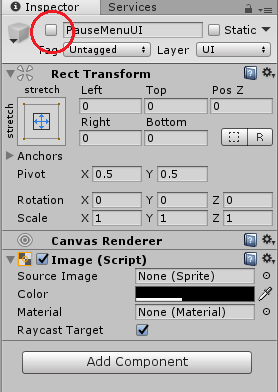
\includegraphics[height=10cm]{images/deactivatePanel.png}
	\caption{Deaktivieren des Panel-Objekts}
	\label{deactivatePanel}
\end{figure}

Daraufhin wird bei dem Canvas-Objekt ein neues Skript hinzugefügt zu sehen in Listing \cref{code:PauseMenu-Skript}.
\begin{lstlisting}[language={[Sharp]C}, caption=PauseMenu-Skript, label=code:PauseMenu-Skript]
using System.Collections;
using System.Collections.Generic;
using UnityEngine;
using UnityEngine.SceneManagement;

public class PauseMenu : MonoBehaviour {

public static bool isPaused = false;
public GameObject PauseMenuUI;

// Update is called once per frame
void Update () {
if(Input.GetKeyDown(KeyCode.Escape))
{
if (isPaused)
{
Resume();
}
else
{
Pause();
}
}
}

public void Resume ()
{
PauseMenuUI.SetActive(false);
Time.timeScale = 1f;
isPaused = false;
}

private void Pause()
{
PauseMenuUI.SetActive(true);
Time.timeScale = 0f;
isPaused = true;
}

public void MainMenu ()
{
SceneManager.LoadScene(0);
}
}
\end{lstlisting}
Beim Script \cref{code:PauseMenu-Skript} gibt es einige Besonderheiten. Als Erstes ist zu sehen, dass alle Eigenschaften der Klasse auf ’public’ gesetzt sind. Dies ist normalerweise untypisch jedoch erleichtert es die Arbeit mit Unity sehr stark da so auch über die GUI des Unity-Editors auf die Eigenschaften der Klasse zugegriffen werden kann und so sich viele neue Möglichkeiten ergeben. Die Eigenschaft ’PauseMenuUI’ bekommt dann das Panel-Objekt zugewiesen.
In der Methode ’Update()’, welche während jedem Frame aufgerufen wird, wird mittels If-Abfrage überprüft ob die Escape-Taste gedrückt wird, wenn ja soll der Status des Spiels abgefragt werden. Ist das Spiel bereits pausiert wird es wieder gestartet und das Panel-Objekt wird wieder deaktiviert. Falls es jedoch läuft wird es gestoppt und das Pause-Menü wird aktiv. Der Stopp wird realisiert durch das Setzen von ’timeScale’ auf 0, wenn es auf 1 gesetzt wird geht das Spiel wieder weiter.
Zu guter Letzt ist noch die Methode des Hauptmenü-Buttons zu sehen, welche ihm später wieder zugewiesen wird. Der ’Back’-Button verwendet die ’Resume()’Methode.


\begin{figure}[H]
	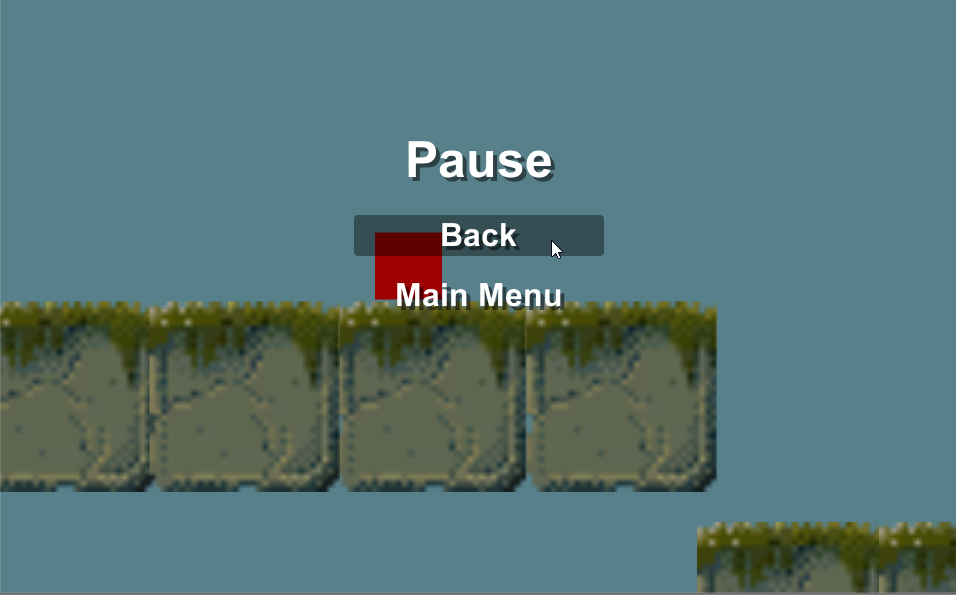
\includegraphics[height=10cm]{images/PauseMenu.png}
	\caption{Pause Menü}
\end{figure}

\section{Leveldesign}
In Unity werden die Einzelnen Level als verschieden Szenen dargestellt.

\begin{figure}[H]
	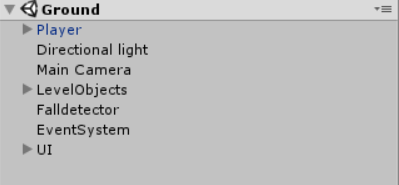
\includegraphics[height=5cm]{images/Ground.png}
	\caption{Hierarchie der Ground Szene}
	\label{hierarchieGround}
\end{figure}
In der Abbildung \ref{hierarchieGround} wird die Hierarchie der Szene dargestellt. Sie stellt alle Objekte der jeweiligen Szene dar. 
\subsection{Player}
Das Level Design ist durch Unity sehr einfach gestaltet. Alle verwenden Graphiken sind nur als Platzhalter verwendet worden.


Für den Player wurde ein Cube-Objekt benutzt.
\begin{figure}[H]
	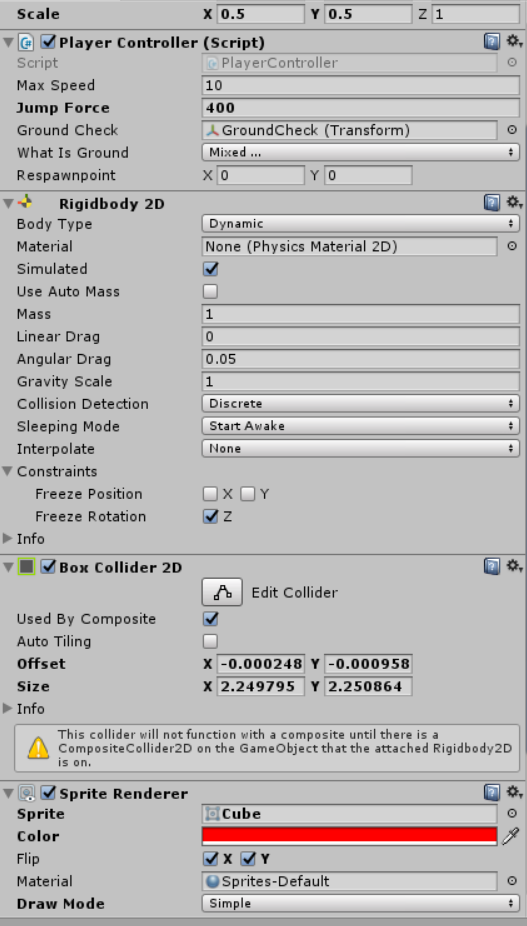
\includegraphics{images/Player.png}
	\caption{Komponenten des Player-Objekts}
	\label{PlayerKomponenten}
\end{figure}
Der Player besteht aus mehreren Komponenten, welche in Abb. \ref{PlayerKomponenten} zu sehen sind. Unter anderem der Box Collider 2D, welcher für die Kollisionen zuständig ist. Der Box Collider muss auf die Größe des Players angepasst werden.
\begin{figure}[H]
	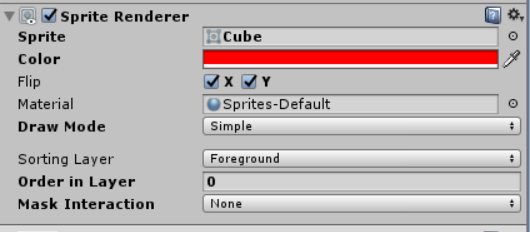
\includegraphics[width=15cm]{images/SpriteRenderer.png}
	\caption{Sprite Renderer Komponente von Player}
\end{figure}
Die Sprite Renderer Komponente ist für die graphische Darstellung des Players verantwortlich. In diesem Fall ist dies eine durchgehend rote Farbe.

\subsection{Directional light}
Damit man als Spieler überhaupt was sehen kann, muss eine Lichtquelle in dem Level platziert werden. Bild von Komponenten In der Light-Komponente können verschiedene Eigenschaften verändert werden, wie zum Beispiel die Intensität, welche für die Stärke des Lichtes verantwortlich ist.
\subsection{Main Camera}
Ein weiterer Faktor zum Sehen des Levels ist die Kamera. Wichtig ist hier, dass man eine geeignete Entfernung wählt, damit man nicht zu wenig oder zu viel sehen kann.
\subsection{LevelObjects}
Bei den LevelObjects handelt es sich um Objekte die Im Level vorkommen, wie der Boden oder Wände. Hierzu werden einzelne Cube-Objekte erschaffen und diese zu Gruppe verbunden. In der Gruppe wird dann der Box Collider 2D hinzugefügt, damit die Objekte eine Kollision mit dem Spieler haben. Auch aber das Ziel zählt unter LevelObjects, wie hier eine Kiste als Platzhalter. Bei der Kiste wurde nur noch ein Skript beigehängt, welches dafür sorgt, dass wenn der Spieler das Ziel erreicht, er zurück zum Level Menü kommt.
\subsection{Falldetector}
Bei dem Falldetector handelt es sich um eine unsichtbares Objekt, welches ebenso einen Box Collider hat. Das Skript, dass dem Player angehängt ist, erkennt ob er dieses Objekt berührt und setzt den Spieler auf die Startposition zurück.
\newpage
\section{Spieler}
\def \currentAuthor {Michael Leitner}
Der Spieler steuert mehrere spielbare Charaktere im Verlauf eines Levels. Damit aber auch die Eingaben des Spielers verwertet werden, werden Skripte benötigt, die diese eingaben auswerten und verwerten. Diese Aufgabe wird von dem PlayerController Skript übernommen. 
\subsection{PlayerController}
Damit der Charakter überhaupt Bewegungen ausführen kann, wurde ihm ein Rigidbody2D-
Container angehängt. 

\begin{figure}[htbp] 
	\centering
	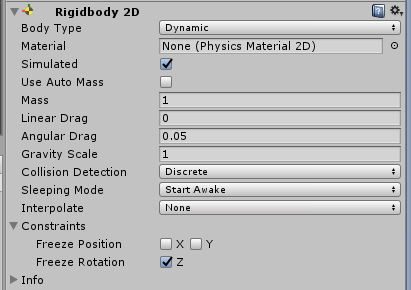
\includegraphics[width=0.7\textwidth]{images/Ridigbody2D.png}
	\caption{Aufbau des Ridigbody2D Containers}
\end{figure}
In diesem Container können verschiedene Eigenschaften, die sich auf den Charakter auswirken, verändert werden. Unter anderem die ’Mass’ Eigenschaft, welche für das Gewicht des Charakters zuständig ist.


\begin{lstlisting}[language={[Sharp]C}, caption=Player-Script]
void FixedUpdate ()
{
grounded = Physics2D.OverlapCircle(groundCheck.position, groundRadius, whatIsGround);

float move = Input.GetAxis("Horizontal");
Rigidbody2D rb = GetComponent<Rigidbody2D>();
rb.velocity = new Vector2(move * maxSpeed, GetComponent<Rigidbody2D>().velocity.y);

if (move > 0 && !faceingRight)
Flip();
else if (move < 0 && faceingRight)
Flip();
}
\end{lstlisting}

Wie schon besprochen, wurde hier die FixedUpdate-Methode verwendet, da eine Bewegung unabhängig von der Framezahl berechnet werden soll. Am Anfang der Methode wird überprüft ob sich der Charakter auf dem Boden befinden. Hierfür wird der Funktion OverlapCircle" die Parameter für den "groundCheck", "groundRadiusünd "whatIsGround" mitgegeben
\begin{itemize}
	\item Das "groundCheckObjekt ist ein unsichtbares Objekt, das dem Charakter angehängt worden ist und dafür zuständig, dass sich der Boden und der "groundCheck" überschneiden.
	\item "groundRadius" legt den Radius fest in dem sich der Boden und "groundCheck" überschneiden müssen, damit die Funktion einen booleschen "true" Wert zurückgibt.
	\item "whatisGround" hat die Funktion, der Funktion zu sagen, welche Objekte überhaupt als Boden zählen.
\end{itemize}
Diese Zeile dient dazu, dass der Charakter springen kann.

Die Zeilen 6-13 sind für die Bewegung zuständig. In Zeile 6 wird der Input des Spielers eingelesen, wobei nur der Input für die horizontale Bewegung wahrgenommen wird. In der Zeile 8 wird dann die Bewegung mittels einer Vektorberechnung ausgeführt. Die Zeilen 10-13 sind für die Änderung der Richtung verantwortlich, wobei beide aber nur die Flip-Methode aufrufen. In der Flip-Methode wird letztendlich nur der Charakter gedreht, damit er sich in eine andere Richtung bewegen kann. Für das Springen des Charakters ist ebenso eine Vektorrechnung verantwortlich, diesmal in vertikaler Richtung.

\section{Kameraführung}
Die Kameraführung wurde einfach gelöst. Die Kamera wurde, auf einer bestimmten Entfernung, an den Charakter gehängt.

\begin{lstlisting}[language={[Sharp]C}, caption=Camera-Script]
public class CameraController : MonoBehaviour {

public GameObject player;

private Vector3 offset;

void Start () {
offset = transform.position - player.transform.position;
}

void LateUpdate () {
transform.position = player.transform.position + offset;
}
}
\end{lstlisting}
Damit die Kamera flüssig den Charakter verfolgt, wurde die LateUpdate-Methode verwendet.

\section{Schalter und Türen}
Für das Öffnen einer Tür, wurde eine Druckplatte verwendet.
\begin{lstlisting}[language={[Sharp]C}, caption=PressurePlate-Script]
void Update ()
{
if ((obj1.transform.position - player.transform.position).magnitude < 1.0f)
{
float step = speed * Time.deltaTime;
Door.transform.position = Vector3.MoveTowards(Door.transform.position, target.position, step);
}
}
\end{lstlisting}

\begin{figure}[H]
	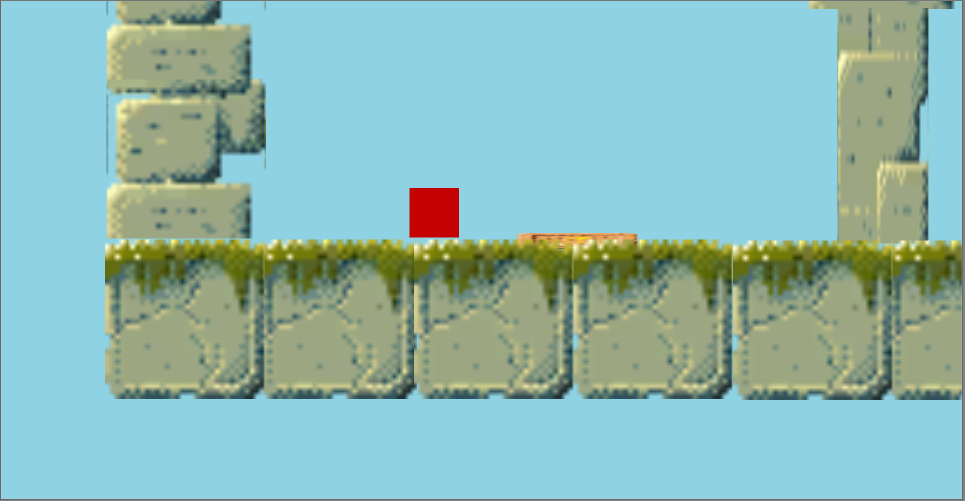
\includegraphics[height=8cm]{images/TuerZu.png}
	\caption{Tür geschlossen}
\end{figure}
Bei dem Skript wird ähnlich wie bei dem PlayerController-Skript(Erkennen ob Player am Boden ist) wird hier überprüft ob sich der Spieler in der nähe der Druckplatte befinden. Ist dies der Fall, wird die Tür zu der "Target"-Position befördert. 
\begin{figure}[H]
	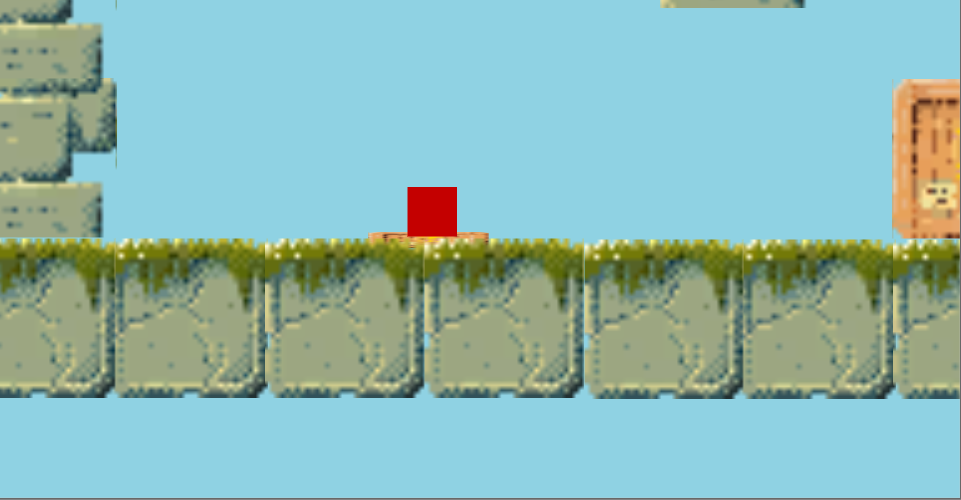
\includegraphics[height=8cm]{images/TuerOffen.png}
	\caption{Tür geöffnet}
\end{figure}

\section{Time Rift}
Das Time Rift-Prinzip ist die grundlegende Funktion in diesem Projekt. Während des ersten Durchlaufes des Spielers, werden in jedem Frame die Koordinaten des Charakters gespeichert.
\begin{lstlisting}[language={[Sharp]C}, caption=TimeRift-Script]
void Update () {
movementSave.addBewegung(new Bewegung(new Koordinatee(posX, posY), new Koordinate(player.transform.position.x, player.transform.position.y)));
posX = player.transform.position.x;
posY = player.transform.position.y;
}
\end{lstlisting}
Dazu wird eine in der Liste "movementSaveline neue Bewegung gespeichert. Die Bewegung wird immer von den alten Koordinaten aus gespeichert. Ist jetzt dann der Durchlauf beendet, so wird das Level zurückgesetzt und die Liste "movementSave" wird und die Liste "restartMovementSave" gespeichert.
\begin{lstlisting}[language={[Sharp]C}, caption=TimeRift-Restart]
private void restart()
{
restartMovementSave.Add(movementSave);
posX = 0;
posY = 0;
count = -1;
restartCount++;
playerCount++;
movementSave = new Bewegungsspeicher();
movementSave.addBewegung(new Bewegung(new Koordinate(0, 0), new Koordinate(0, 0)));
}
\end{lstlisting}
Ebenso werden die andere Werte gesetzt, wie z.B.: Die Startkoordinaten.
\begin{lstlisting}[language={[Sharp]C}, caption=TimeRift-Bewegungsspeicher]
public class Bewegungsspeicher
{
private ArrayList bewegungslist = new ArrayList();

public void addBewegung(Bewegung bewegung)
{
bewegungslist.Add(bewegung);
}

public Bewegung getBewegung(int zahl)
{
if ((bewegungslist.Count - 1) >= zahl)
{
return (Bewegung) bewegungslist[zahl];
}

return null;
}

public ArrayList getArray()
{
return bewegungslist;
}
}
\end{lstlisting}
In der Klasse "Bewegungsspeicher" wird die ArrayList für die Bewegungen initialisiert.
Damit im zweiten Durchlauf des Levels, die erste Spielfigur dieselben Bewegungen macht, werden in jedem Frame die Koordinaten aus der ArrayList gelesen und bei der Figur gesetzt.


\chapter{Tests}

\section{Systemtests} 
\subsection{Einführung}
Nachfolgend sind vier tabellarisch dargestellte Testfälle beschrieben, welche grundlegende Funktionen des Projekts Darstellen und deren Funktionalität gewährleisten sollen.
\subsection{Testfälle}
\def \currentAuthor {Lukas Vogel}
\begin{table}
	
\renewcommand{\arraystretch}{1.5}
\begin{tabular}{|p{3.5cm}|p{11cm}|}
	
	\hline 
	\textbf{Nummer} & 1 \\ 
	\hline 
	\textbf{Name} & {\large Bewegungssteuerung} \\ 
	\hline 
	\textbf{Beschreibung} & 
	Es soll gewährleistet werden, dass die Steuerung der Spielfigur mittels der unten angegebenen Tasten sowie deren Kombination miteinander wie gewünscht funktioniert.  \\ 
	\hline 
	\textbf{Vorbedingung} & 
	\begin{itemize}
		\setlength{\itemsep}{1pt}
		\setlength{\parskip}{0.5pt}
		\item Spiel muss gestartet sein
		\item Level muss gewählt sein
	\end{itemize} \\ 
	\hline 
	\textbf{Tester} & Lukas Vogel \\ 
	\hline 
	\textbf{Datum} & 8.5.2018 \\ 
	\hline 
	\textbf{Vorgehen} & 
	\textit{Soll-Verhalten:}
	\begin{itemize}
		\setlength{\itemsep}{1pt}
		\setlength{\parskip}{0.5pt}
		\item A --> Bewegung der Spielfigur nach links.
		\item D --> Bewegung der Spielfigur nach rechts.
		\item Leertaste --> Vertikale Bewegung der Spielfigur nach oben.
		\item A + Leertaste --> Eine gemischte Bewegung die Horizontal nach links und Vertikal nach oben geht (Sprung nach links).
		\item D + Leertaste --> Eine gemischte Bewegung die Horizontal nach rechts und vertikal nach oben geht (Sprung nach rechts) \newline
	\end{itemize}  
	
	
	\textit{Ist Verhalten:}
	\begin{itemize}
		\setlength{\itemsep}{1pt}
		\setlength{\parskip}{0.5pt}
		\item A --> Spielfigur bewegt sich nach links.
		\item D --> Spielfigur bewegt sich nach rechts.
		\item Leertaste --> Spielfigur bewegt sich vertikal nach oben.
		\item 	A + Leertaste --> Sprung nach links.
		\item D + Leertaste --> Sprung nach rechts.
	\end{itemize}\\ 
	\hline 
	\textbf{Erfolgskriterien} & 
	\textit{Gewünschtes Verhalten:}
	\begin{itemize}
		\setlength{\itemsep}{1pt}
		\setlength{\parskip}{0.5pt}
		\item Flüssige Bewegung ohne Stopps
		\item Bedingte Beeinflussung des Verhaltens durch die Physik-Engine
		\item Tatsächliche Bewegung durch Tastendruck
	\end{itemize} \\ 
	\hline 
\end{tabular} 
\caption{Testfall 1: Bewegungssteuerung}
\end{table}

\begin{table}

	\renewcommand{\arraystretch}{1.5}
	\begin{tabular}{|p{3.5cm}|p{11cm}|}
		
		\hline 
		\textbf{Nummer} & 2 \\ 
		\hline 
		\textbf{Name} & {\large Levelabschluss} \\ 
		\hline 
		\textbf{Beschreibung} & 
		Es soll gewährleistet werden, dass der Spieler beim Abschließen des Levels in eine Übersicht (Level-Übersicht) gebracht wird. Durch das Öffnen der Level-Übersicht kann der User entscheiden ob er ein anders Level öffnen will oder mittels Button ins Hauptmenü der Anwendung wechseln. \\ 
		\hline 
		\textbf{Vorbedingung} & 
		\begin{itemize}
			\setlength{\itemsep}{1pt}
			\setlength{\parskip}{0.5pt}
			\item Spiel muss gestartet sein
			\item Level muss gewählt sein
			\item Spieler muss Ende des Levels erreichen
		\end{itemize} \\ 
		\hline 
		\textbf{Tester} & Lukas Vogel \\ 
		\hline 
		\textbf{Datum} & 8.5.2018 \\ 
		\hline 
		\textbf{Vorgehen} & 
		\textit{Soll-Verhalten:}
		\begin{itemize}
			\setlength{\itemsep}{1pt}
			\setlength{\parskip}{0.5pt}
			\item Beim Levelabschluss kommt ein Overlay, das 2 Möglichkeiten bieten (Nächstes Level, Hauptmenü)
			\item Wird einer der Levelbuttons (nummerierte Quadrate) betätigt, startet das gewünschte Level. 
			\item Der Button „Back“ bringt den Spieler in das Hauptmenü des Spieles. \newline
		\end{itemize}  
		
		
		\textit{Ist Verhalten:}
		\begin{itemize}
			\setlength{\itemsep}{1pt}
			\setlength{\parskip}{0.5pt}
			\item Wechsel in die Levelübersicht nach Abschluss des Levels
			\item Wird Levelbutton gedrückt startet richtiges Level
			\item Back-Button öffnet Hauptmenü 
		\end{itemize}\\ 
		\hline 
		\textbf{Erfolgskriterien} & 
		\textit{Gewünschtes Verhalten:}
		\begin{itemize}
			\setlength{\itemsep}{1pt}
			\setlength{\parskip}{0.5pt}
			\item 	Der Spieler soll durch das Overlay die Auswahlmöglichkeit haben, weiter zu spielen oder zurück ins Hauptmenü zu navigieren.
		\end{itemize} \\ 
		\hline 
	\end{tabular} 
	\caption{Testfall 2: Levelabschluss}
\end{table}
\newpage
\def \currentAuthor {Michael Leitner}
\begin{table}

	\renewcommand{\arraystretch}{1.5}
	\begin{tabular}{|p{3.5cm}|p{11cm}|}
		
		\hline 
		\textbf{Nummer} & 3 \\ 
		\hline 
		\textbf{Name} & {\large Tod der Spielfigur durch Fall} \\ 
		\hline 
		\textbf{Beschreibung} & 
		Bei einem Fehler des Spielers, indem er durch falsches Steuern des Charakters aus der Spielwelt fällt, wird der Charakter wieder zur Startposition zurückgesetzt. \\ 
		\hline 
		\textbf{Vorbedingung} & 
		\begin{itemize}
			\setlength{\itemsep}{1pt}
			\setlength{\parskip}{0.5pt}
			\item Spiel muss gestartet sein
			\item Level muss gewählt sein
			\item Spieler fällt aus der Spielwelt
		\end{itemize} \\ 
		\hline 
		\textbf{Tester} & Michael Leitner \\ 
		\hline 
		\textbf{Datum} & 8.5.2018 \\ 
		\hline 
		\textbf{Vorgehen} & 
		\textit{Soll-Verhalten:}
		\begin{itemize}
			\setlength{\itemsep}{1pt}
			\setlength{\parskip}{0.5pt}
			\item Charakter wird ab einer bestimmten Grenze („Deathzone“) an den Startpunkt des Levels zurückgesetzt („Respawn“).\newline
		\end{itemize}  
		
		
		\textit{Ist Verhalten:}
		\begin{itemize}
			\setlength{\itemsep}{1pt}
			\setlength{\parskip}{0.5pt}
			\item Respawn der Spielfigur funktioniert. 
		\end{itemize}\\ 
		\hline 
		\textbf{Erfolgskriterien} & 
		\textit{Gewünschtes Verhalten:}
		\begin{itemize}
			\setlength{\itemsep}{1pt}
			\setlength{\parskip}{0.5pt}
			\item Durch das zurücksetzten des Charakters soll ein reibungsloses weiterspielen möglich sein.
		\end{itemize} \\ 
		\hline 
	\end{tabular} 
	\caption{Testfall 3: Tod der Spielfigur durch Fall}
\end{table}

\begin{table}

	\renewcommand{\arraystretch}{1.5}
	\begin{tabular}{|p{3.5cm}|p{11cm}|}
		
		\hline 
		\textbf{Nummer} & 4 \\ 
		\hline 
		\textbf{Name} & {\large Schalter zum Öffnen einer Tür} \\ 
		\hline 
		\textbf{Beschreibung} & 
		Beim Betätigen des Schalters mittels der Spielfigur, soll eine Tür/Passage geöffnet werden, welche für den weiteren Spielverlauf wichtig ist. \\ 
		\hline 
		\textbf{Vorbedingung} & 
		\begin{itemize}
			\setlength{\itemsep}{1pt}
			\setlength{\parskip}{0.5pt}
			\item Spiel muss gestartet sein
			\item Level muss gewählt sein
			\item Spieler ist bei einem Schalter
		\end{itemize} \\ 
		\hline 
		\textbf{Tester} & Michael Leitner \\ 
		\hline 
		\textbf{Datum} & 8.5.2018 \\ 
		\hline 
		\textbf{Vorgehen} & 
		\textit{Soll-Verhalten:}
		\begin{itemize}
			\setlength{\itemsep}{1pt}
			\setlength{\parskip}{0.5pt}
			\item Spieler bewegt Spielfigur auf den Schalter
			\item Tür öffnet sich, sobald der Schalter betätigt wurde.\newline
		\end{itemize}  
		
		
		\textit{Ist Verhalten:}
		\begin{itemize}
			\setlength{\itemsep}{1pt}
			\setlength{\parskip}{0.5pt}
			\item Spieler benutzt Schalter und Tür geht auf. 
		\end{itemize}\\ 
		\hline 
		\textbf{Erfolgskriterien} & 
		\textit{Gewünschtes Verhalten:}
		\begin{itemize}
			\setlength{\itemsep}{1pt}
			\setlength{\parskip}{0.5pt}
			\item Durch das Öffnen der Tür sollen neue Gebiete des Levels erschlossen werden, um auch letztendlich das Level abzuschließen zu können
		\end{itemize} \\ 
		\hline 
	\end{tabular} 
	\caption{Testfall 4: Schalter zum Öffnen einer Tür}
\end{table}


\chapter{Projektevaluation}
\def \currentAuthor {Lukas Vogel}
\section{Arbeitsaufwand}
Während der Bearbeitung der Diplomarbeit, lernten wir schnell, dass wir den Arbeitsaufwand des Projektes unterschätzt hatten, am besten wäre es daher, wenn man sich während den verschiedenen Ferien mindestens für mehrere Tage getroffen hätte und dann intensiv gearbeitet hätte. Schlussendlich ist das Projekt zwar trotzdem fertiggestellt worden und es erfüllt auch die gewünschten Anforderungen, jedoch war so viel mehr Arbeit zusätzlich zum normalen Schulalltag nötig.
\section{Zusammenarbeit}
Die Zusammenarbeit des Teams war nie ein Problem, die einzige Komplikation, die wir hatten, war das Ausfallen eines Teammitglieds. Dies führte zu einer erneuten Aufteilung der Aufgaben und zu einer Umstrukturierung des Projektteams. Als Resultat ist der Arbeitsaufwand stark gestiegen und das Projekt war ein noch größere Herausforderung. 

Wichtig ist es noch anzumerken, dass bei der Zuordnung der Themen keine Probleme auftraten, da jeder im Team seinen Wunschschwerpunkt ohne Diskussion bekam. Dies ist darauf zurück zu führen, dass wir diesbezüglich unterschiedlich sind und bei diesem Projekt die Themenauswahl passend zu unseren Persönlichkeiten war.

\section{Zeitmanagement}
Die größte Schwierigkeit war das Zeitmanagement, da das gesamte Team sich nicht nur auf die Bearbeitung der Diplomarbeit konzentrieren konnte, sondern zusätzlich noch die benötigten schulischen Leistungen erbringen musste. Dies führte des Öfteren zu Komplikationen und somit auch zu zeitlichen Verschiebungen von Meilensteinen. Durch Teamarbeit und Arbeitsaufteilung konnte jedoch auch diese Herausforderung gemeistert werden und das Projekt dennoch mit ausreichender Zeit fertig gestellt werden.

\section{Produktevaluierung}
\textbf{Sollzustand}\newline
Es soll ein Spiele-Prototyp entwickelt, der die vorgegebenen Funktionen realisiert. Das Spiel wird vollständig spielbar sein und einige Levels enthalten, die das Spielprinzip voll zur Geltung bringen. Die Software wird in einer Beta-Phase mit Usern getestet, deren Feedback zur Verbesserung des Spiels verwendet wird. Das Spiel wird als voll funktionsfähiges Spiel an den Auftraggeber übergeben.

\textbf{Istzustand}\newline
Es wurde ein Prototyp entwickelt, der alle vorgegebenen Funktionen realisierte. Das Spiel ist vollständig spielbar und ist mit 4 Level ausgestattet. In diesen Level kommt das grundlegende Spielprinzip zur Geltung. Es wurde auf die Beta-Phase verzichtet, aus dem Grund, dass keine Zeit mehr für einen Durchlauf einer Beta-Testphase sowie die Einarbeitung der Ergebnisse des Feedbacks, war. Wegen dem Verlassen eines Projektmitgliedes wurde bei dem Spiel gänzlich auf Soundeffekte und Hintergrundmusik verzichtet. Ebenso wurde die Grafik sehr primitiv gehalten, da das Erstellen von neuen Grafiken sehr aufwendig ist und wir dafür eine zusätzliche Einarbeitungsphase benötigt hätten.

\section{Kosten}
Kosten sind für das Projekt insofern keine entstanden, da wir die benötigte Software für die Entwicklung komplett kostenlos bekommen haben. Die einzigen Kosten waren Zeit und Arbeit somit sind keine Ausgaben entstanden.

\section{Erfahrungen}
Besonders hervorzuheben ist die Vielfalt an neuen Erfahrungen, die wir während des Projektes sammeln konnten. Wir lernten den gesamten Umfang eines Projekts kennen und welche Arbeitsschritte für ein solches Unterfangen notwendig sind, sei es nur die ständige Kommunikation mit den Teammitgliedern bis zur Fertigung einer umfangreichen Projektdokumentation.

\section{Fazit}
Abschließend ist zu sagen, dass es ein sehr spannendes Projekt war, welches uns nicht nur einmal forderte. Wir lassen uns die Möglichkeit offen NeXt noch weiter zu entwickeln und vielleicht sogar eine marktfähige Version zu produzieren.
\chapter{Zusammenfassung}
\section{Resümee}
\subsection{Resümee (Leitner Michael)}
Die Entwicklung eines Spieles war ein größerer Aufwand als erwartet.
Gründe dafür sind:

\begin{enumerate}
	\item Für die ausgewählte Engine war eine intensivere Einarbeitung in die Dokumentation notwendig, um auch die Engine ohne Probleme verwenden zu können.
	\item Der Absprung eines Projektmitgliedes hatte uns mehr Arbeit beschert, aber durch Absprache mit dem Projektpartner und Projektbetreuer, wurde der Projektumfang angepasst.
	\item Das komplette Diplomprojekt neben dem normalen Schulalltag durchzuführen und zu erarbeiten, war ebenso ein Faktor, der sich schwer auf das Zeitmanagement gelegt hat.
\end{enumerate}
	
Letztendlich ist aber alles im Projekt, mehr oder weniger, gut verlaufen. Des Weiteren habe ich viel für die Spiele Entwicklung gelernt, dass ich für zukünftige Projekte (ob privat oder beruflich) anwenden kann. Die Arbeitsaufteilung war zwischen Lukas und mir sehr gerecht und beide hatten ungefähr den gleichen Aufwand. Für alle, die ein Spiel entwickeln möchten, gebe ich nur einen Tipp auf dem Weg: „Plant euch genug Zeit ein. Es hat einen Grund, warum so viele Veröffentlichungen von Spiele verschoben werden.“.

\subsection{Resümee (Vogel Lukas)}
Während der Diplomarbeit lernte ich den Ablauf eines Projekts hautnah kennen und konnte somit viele wertvolle Erfahrungen sammeln, welche mir sicherlich auch in Zukunft helfen werden.
Die ersten Neuerungen für mich waren die vielen verschieden Programme, die wir im Laufe unsers Projekts verwendeten. Eine Software, die für mich komplett neu war, war Latex mit der wir die Diplomarbeit dann geschrieben haben. Ein Textverarbeitungsprogramm in der man die Formatierung „programmiert“ war etwas Ungewohntes, jedoch ist das Programm perfekt auf wissenschaftliche Arbeiten wie Diplomarbeiten zugeschnitten und zeigte uns einige Vorteile gegenüber anderer Applikationen.
Mitten während des Projekts lernten wir wie wichtig es ist immer einen Plan-B zu haben, da eine Teammitglied die das IT-Kolleg frühzeitig beendete und wir somit ein Teammitglied weniger waren. Dies hatte zur Folge, dass wir die Aufteilung sowie den Umfang des Projekts noch einmal komplett überdenken mussten.
Besonders interessant war das Kennenlernen der Spieleentwicklung und dadurch einen Überblick zu bekommen wieviel Arbeit hinter so einer Software steckt. Das erste große Thema war die Einarbeitung in eine komplett fremde Programmierumgebung. Natürlich hatten wir mit der Programmiersprache C\# schon während unser Unterrichts zu tun, jedoch ist das Programmieren mit C\# in Kombination mit der Spiele-Engine Unity nochmal etwas ganz anderes. Was mir dabei aber auffiel war, dass nach der Lernphase und der Eingewöhnungszeit in die neue Entwicklungsumgebung von Unity, auch hier wieder einige Parallelen mit den im Unterricht besprochen Themen zu ziehen waren. Man darf aber an dieser Stelle nicht glauben, dass das entwickeln mit Unity dem normalen Programmieren von Anwendungen stark ähnelt, da Unity auf eine ganz eigene Art funktioniert.
Die größte Aufgabe war eindeutig das Zeitmanagement. Das Problem war, zusätzlich zu den vielen Unterrichtseinheiten und die Zeit, die für das Lernen oder das erledigen anderer wichtiger schulischer Tätigkeiten war, noch Zeit für das Projekt zu finden. Diese Schule fordert einen mehr als alle anderen die ich zuvor besucht habe und zusätzlich kommt dann noch die Diplomarbeit hinzu. Es gab nicht nur einmal den Punkt, an dem ich nicht mehr wusste, wie ich alles erledigen sollte. Abschließend ist nur zu sagen das es eine besondere Herausforderung war diese Diplomarbeit zu erstellen und ich sehr viel fürs Leben dazugelernt habe.
